%!TEX root = ../../../adrien_gomar_phd.tex

In contrast to turbomachinery applications, convergence
on CROR configurations
in terms of harmonics has been observed to be
slow on some configurations.

\subsection{Presentation of the cases}

To investigate this issue, two CROR configurations are studied at
different operating conditions:
\begin{enumerate}
\item a Mock-up CROR (noted \mockup) designed by Safran to be
  investigated in a wind tunnel (\emph{i.e.} ground condition:
  $P_i=101,300$~Pa and $T_i=293$~K). Two regimes are considered
  representative of low and high-speed conditions (different rotation
  speeds and blade angles). This configuration is the one
  studied in this thesis and detailed results will be given 
  in Chapters~\ref{cha:dream_ls_isolated} and~\ref{cha:dream_hs_isolated},
\item the Airbus-designed AI-PX7 CROR (noted \aipx) at cruise
  condition: high-speed 
  and flight level (\emph{i.e.}  $P_i=23,842$~Pa and
  $T_i=219.6$~K). This configuration has been studied by
  \citet{ThesisFrancois} in his PhD thesis and is used
  here for comparison.
\end{enumerate}

\subsection{Results of HB computations}

Figures~\ref{fig:mulscv},
\ref{fig:muhscv} and \ref{fig:aipx7cv} show the non-dimensional
entropy at 75\% span computed by the HB method for the three
configurations. The \mockup-LS configuration has the fastest
convergence. There are indeed some spurious entropy waves downstream the blade
row interface for $N=1$ and 2 but none are observed
starting $N=4$.
\begin{figure}[htp]
  \centering
  \subfigure[$N=1$]{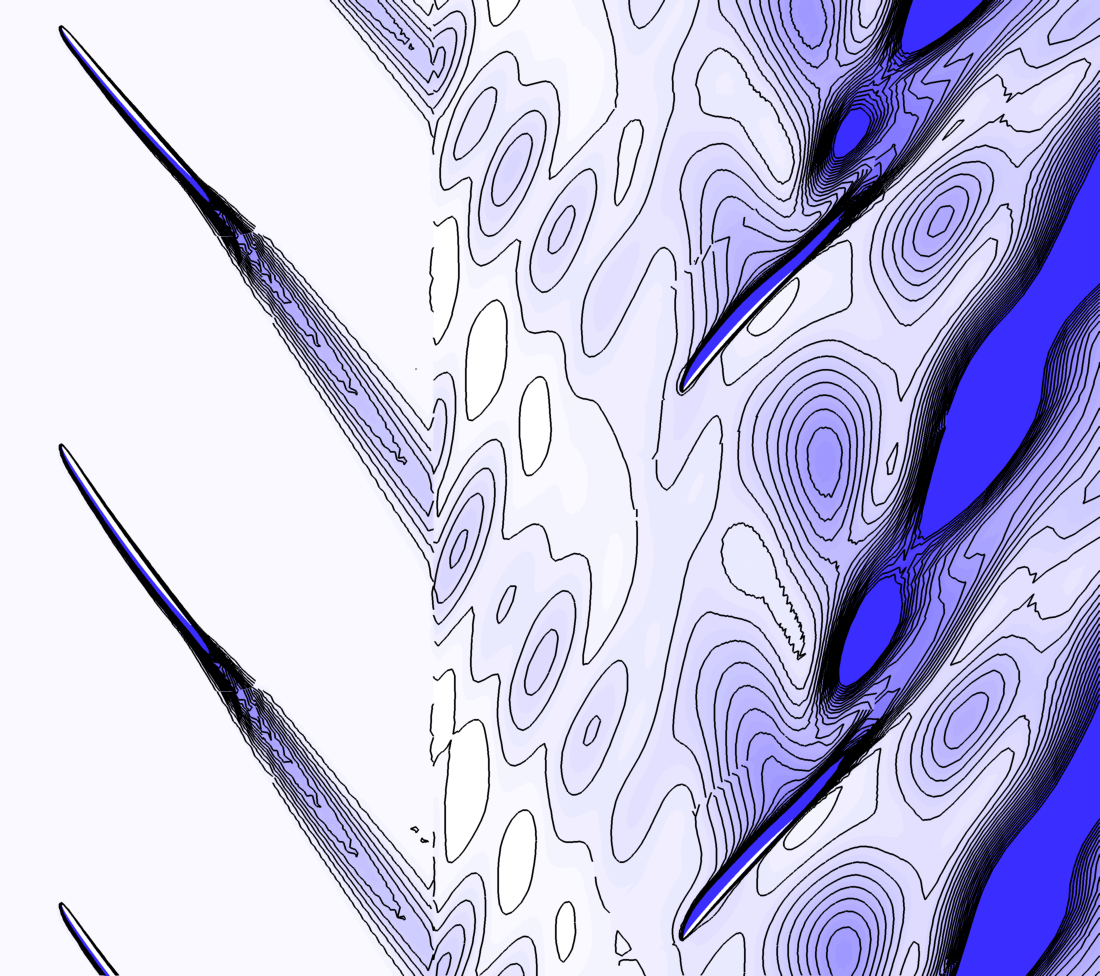
\includegraphics[width=.3\textwidth]{dream_LS_N01_entropy_75.jpg}}
  \subfigure[$N=2$]{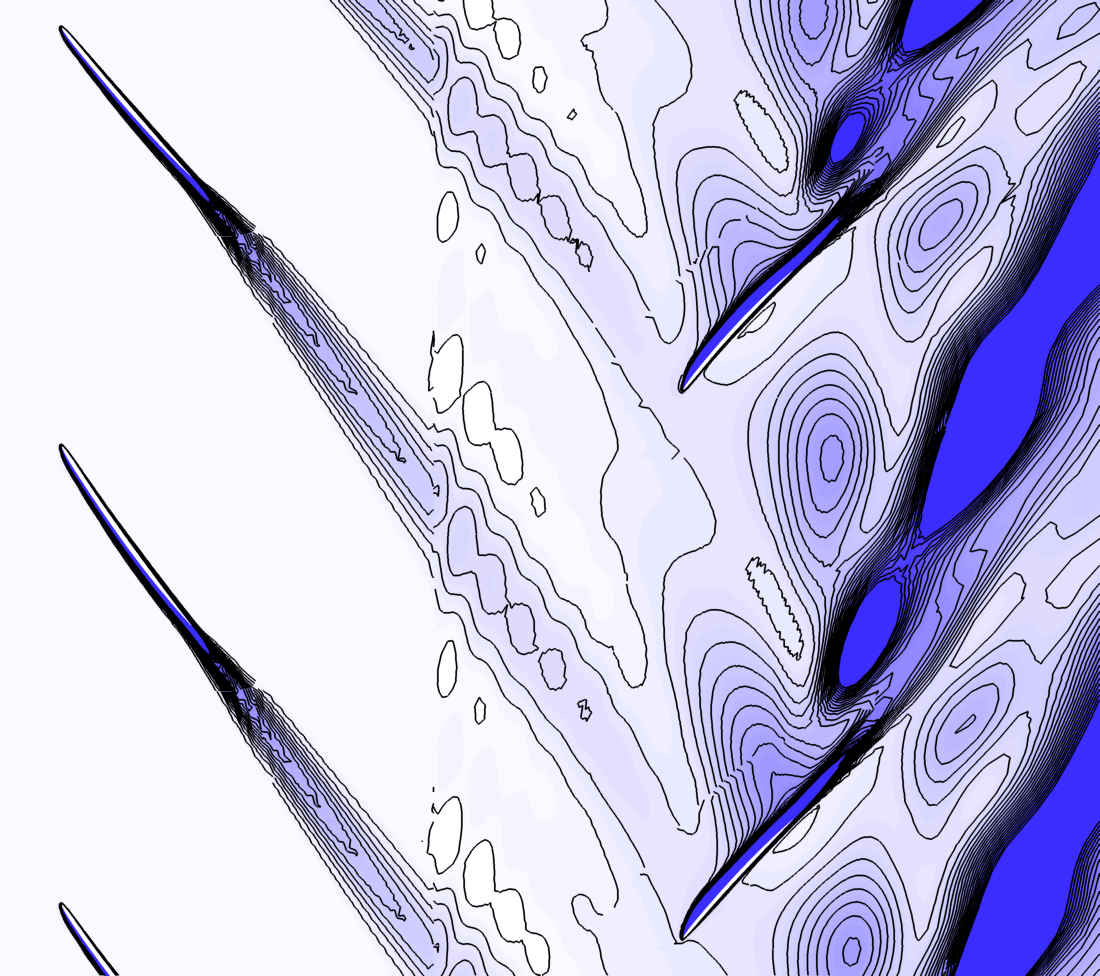
\includegraphics[width=.3\textwidth]{dream_LS_N02_entropy_75.jpg}}
  \subfigure[$N=3$]{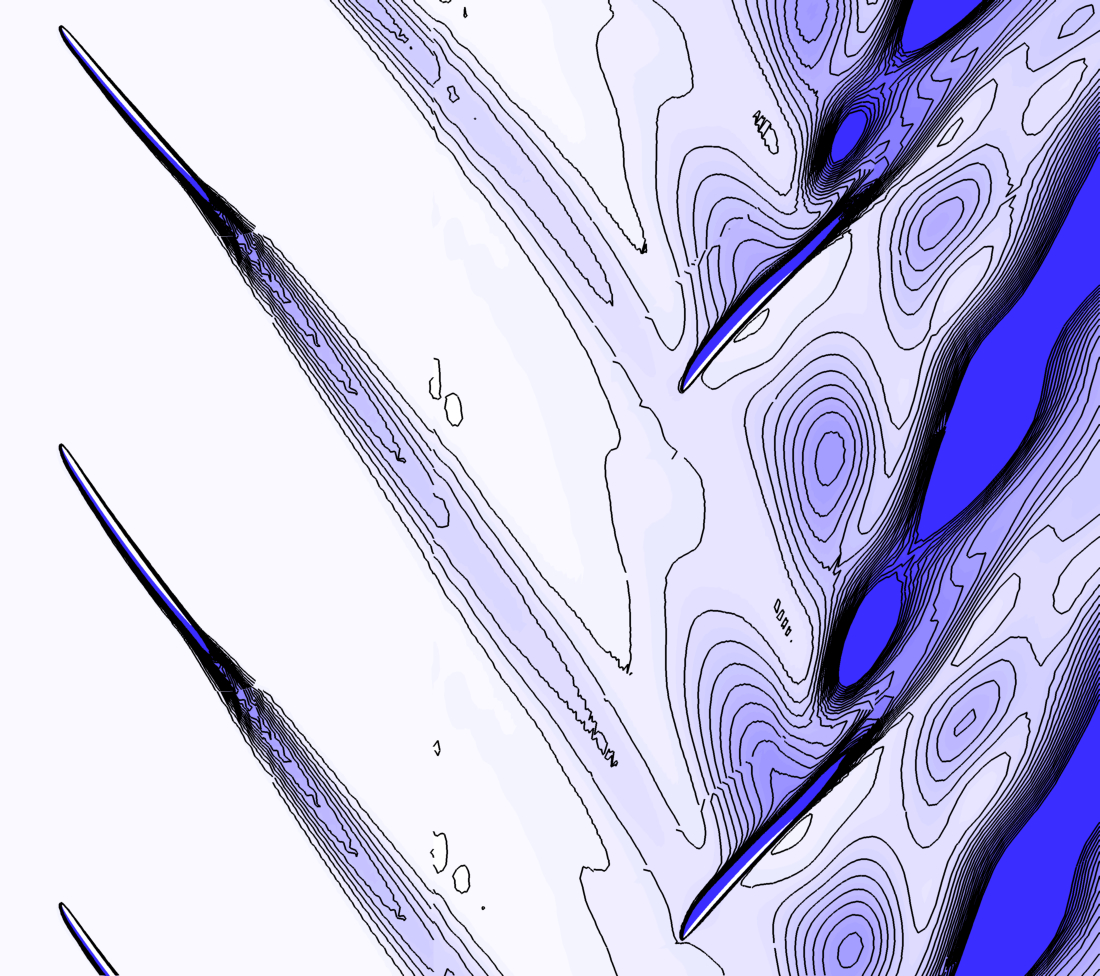
\includegraphics[width=.3\textwidth]{dream_LS_N03_entropy_75.jpg}}
  \subfigure[$N=4$]{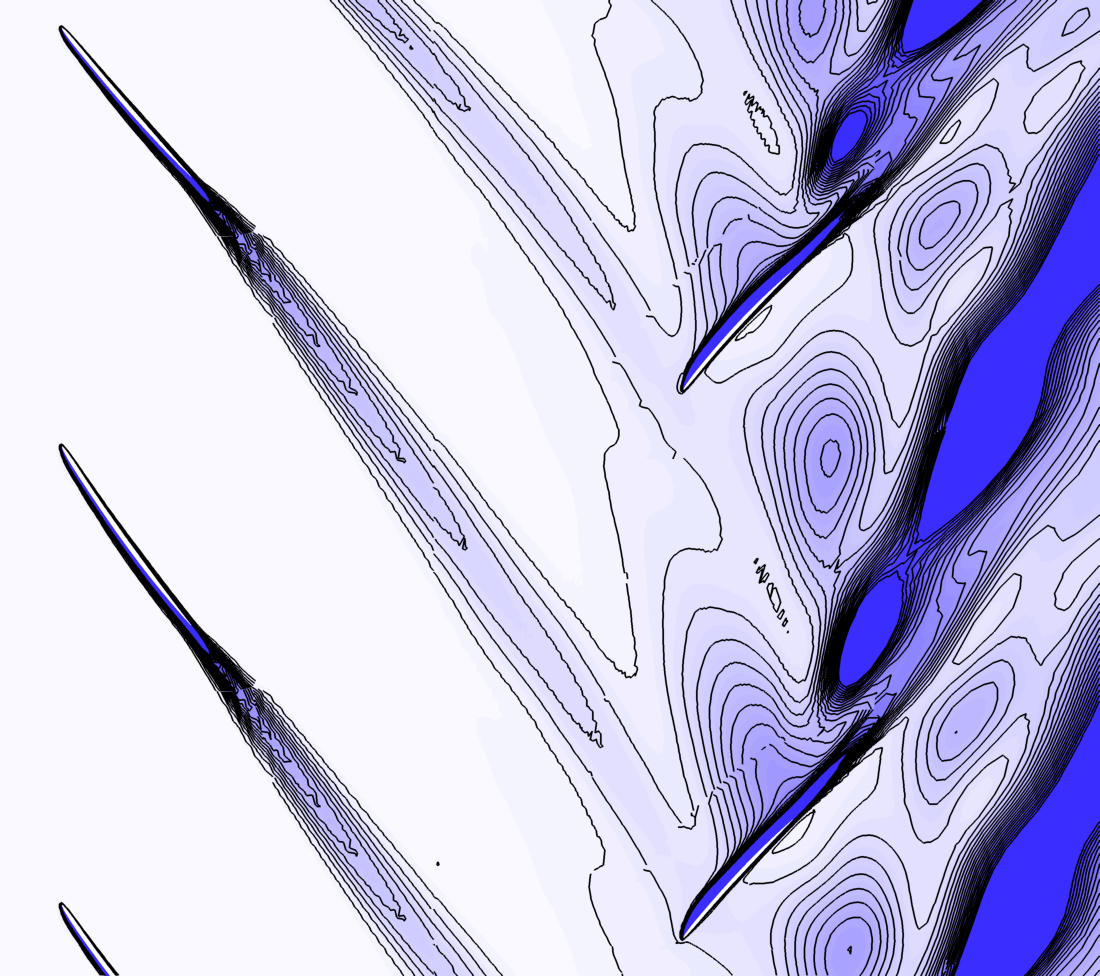
\includegraphics[width=.3\textwidth]{dream_LS_N04_entropy_75.jpg}}
  \subfigure[$N=5$]{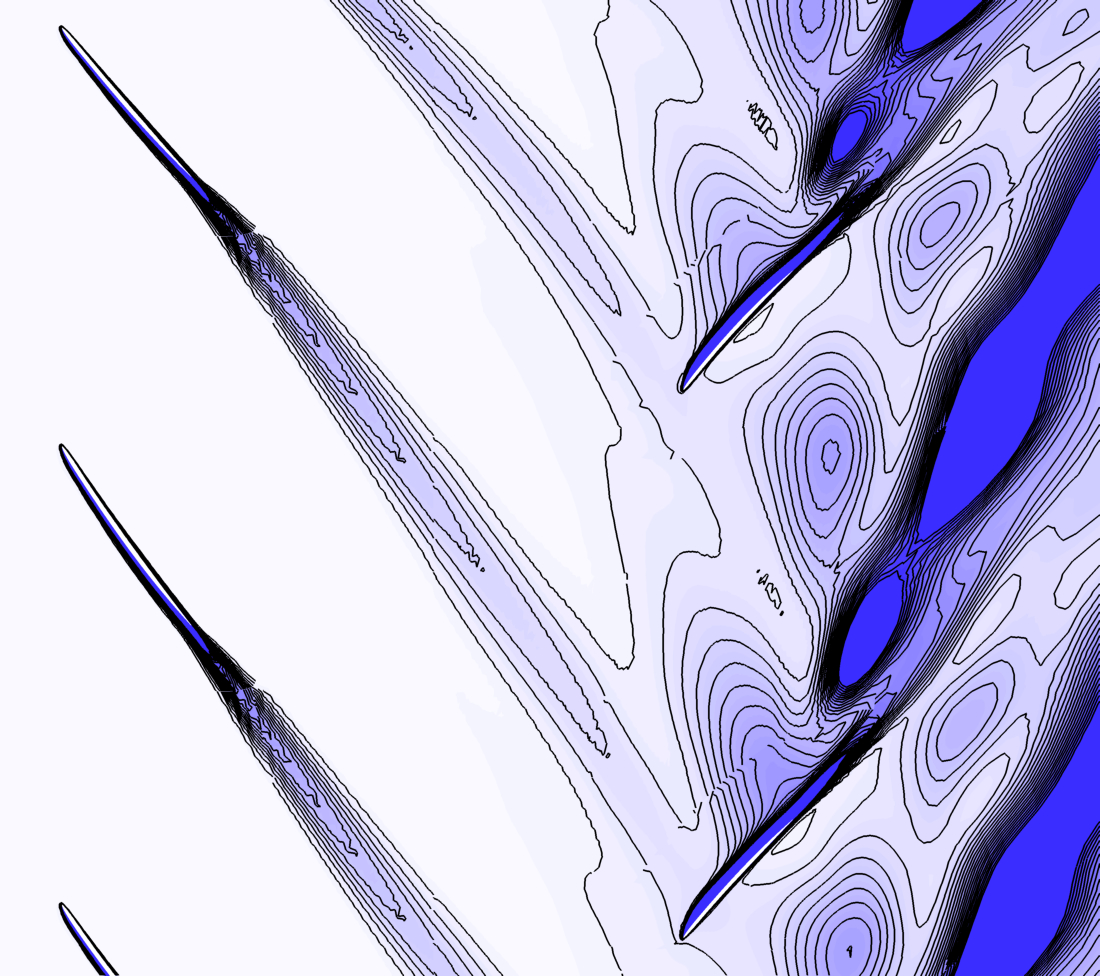
\includegraphics[width=.3\textwidth]{dream_LS_N05_entropy_75.jpg}}
  \subfigure[$N=6$]{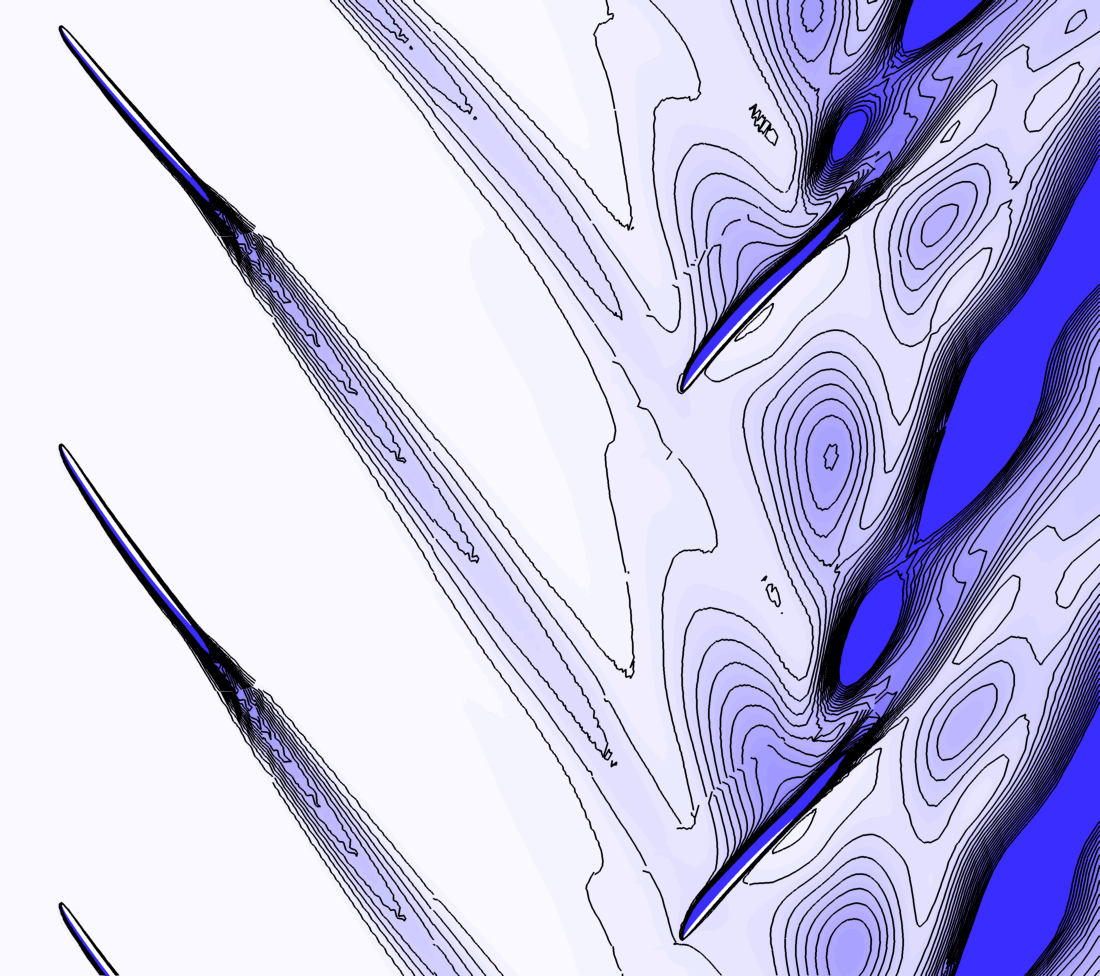
\includegraphics[width=.3\textwidth]{dream_LS_N06_entropy_75.jpg}}
  \caption{\mockup-LS convergence -- Non-dimensional entropy at 75\% span.}
  \label{fig:mulscv}
\end{figure}

For the \mockup-HS configuration, one can
observe in Fig.~\ref{fig:muhscv}(g) that the $N=7$~HB~computation still
presents some spurious waves downstream the interface. It becomes
negligible for a finer sampling. The main difference with the \mockup-LS
configuration is the blade angle. By comparing Fig.~\ref{fig:mulscv}
and Fig.~\ref{fig:muhscv}, one can observe that the blade angle is
higher in the high-speed case. Therefore, even if the wake is of similar
thickness downstream the front rotor, it impacts the axial blade row
interface with a higher angle and therefore looks thinner: Assuming
the flow angle downstream the trailing edge is the same as the
blade incidence angle~$\xi$, the wake thickness observed by the blade row
interface $L_{itf}$ is 
\begin{equation}
  L_{itf}=\frac{L}{\cos(\xi)}.
\end{equation}
When $\xi$ rises from low-speed to high-speed configuration, $L$ will
remain almost constant but $L_{itf}$ will decrease and the spectrum
becomes richer.
\begin{figure}[htp]
  \centering
  \subfigure[$N=1$]{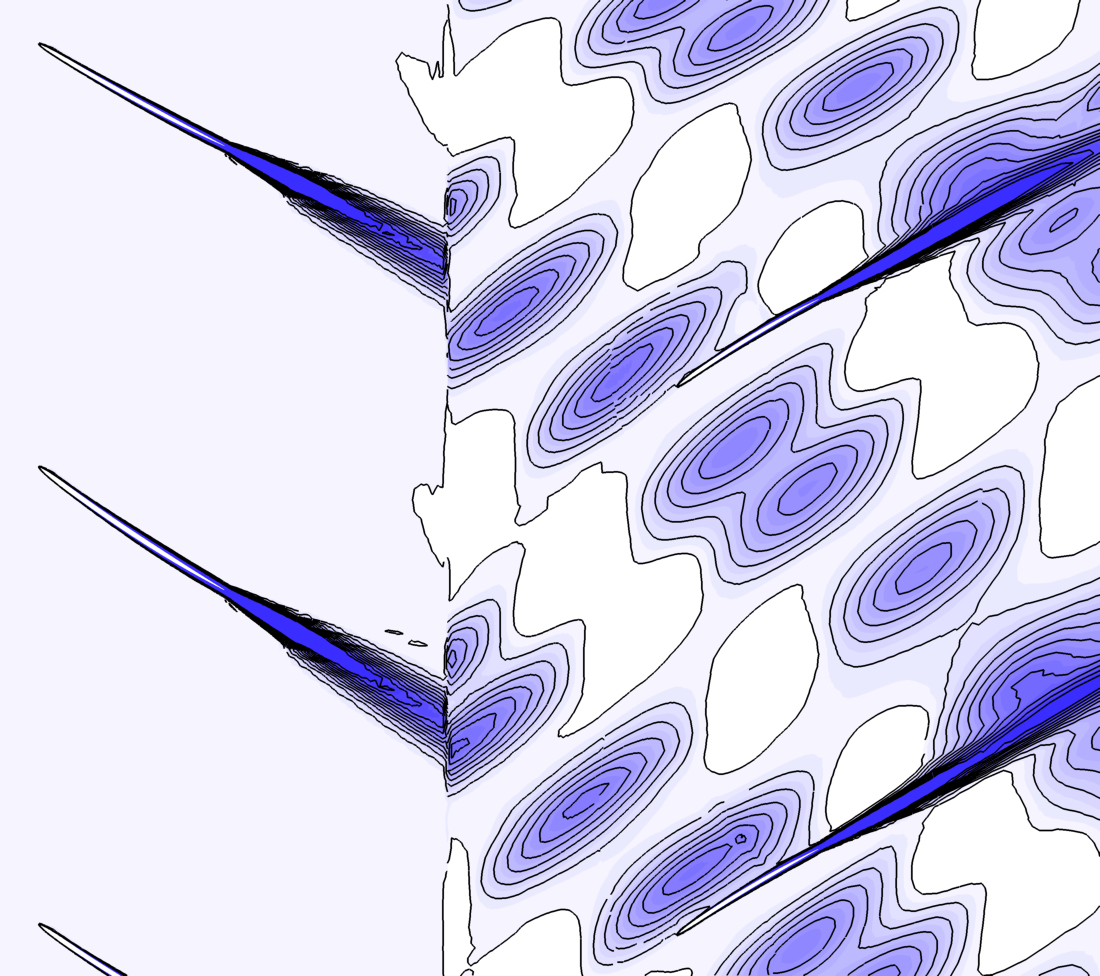
\includegraphics[width=.3\textwidth]{dream_HS_N01_entropy_75.jpg}}
  \subfigure[$N=2$]{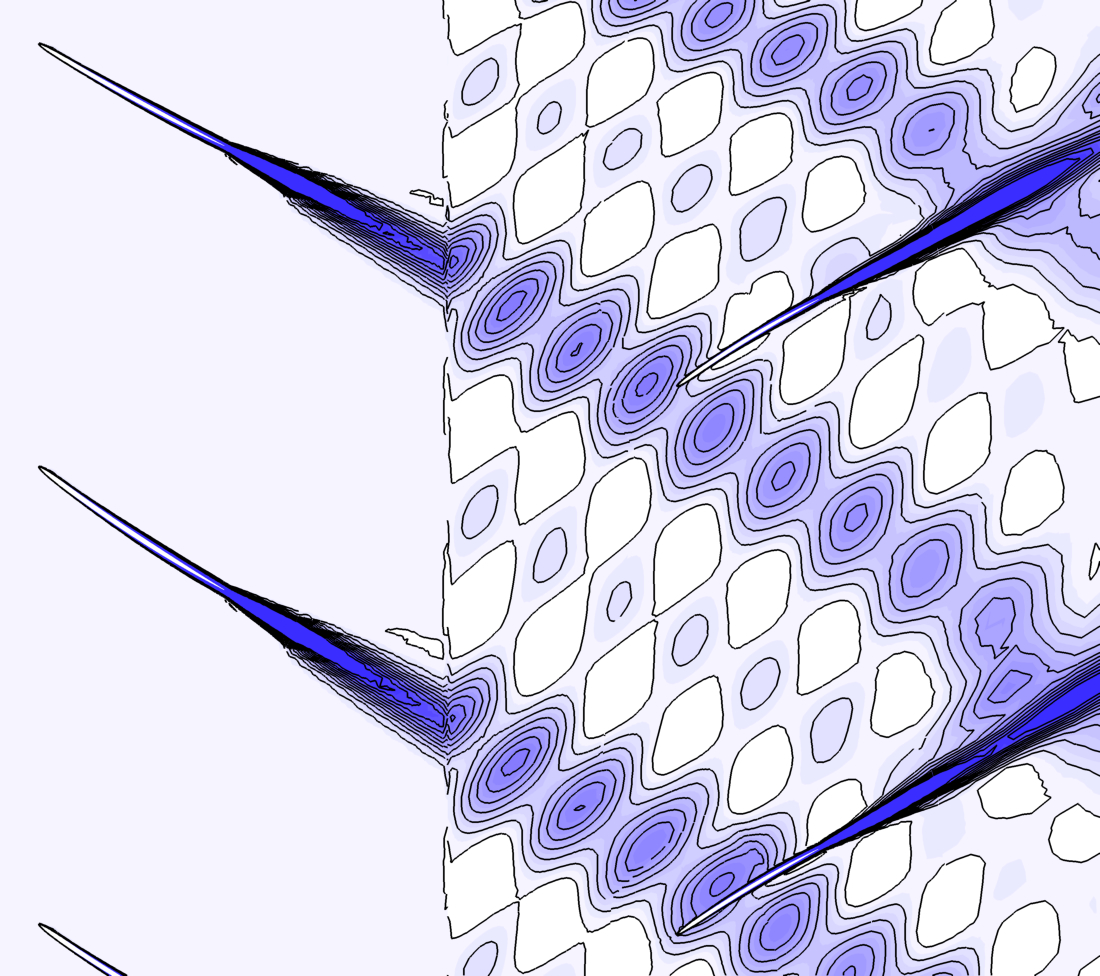
\includegraphics[width=.3\textwidth]{dream_HS_N02_entropy_75.jpg}}
  \subfigure[$N=3$]{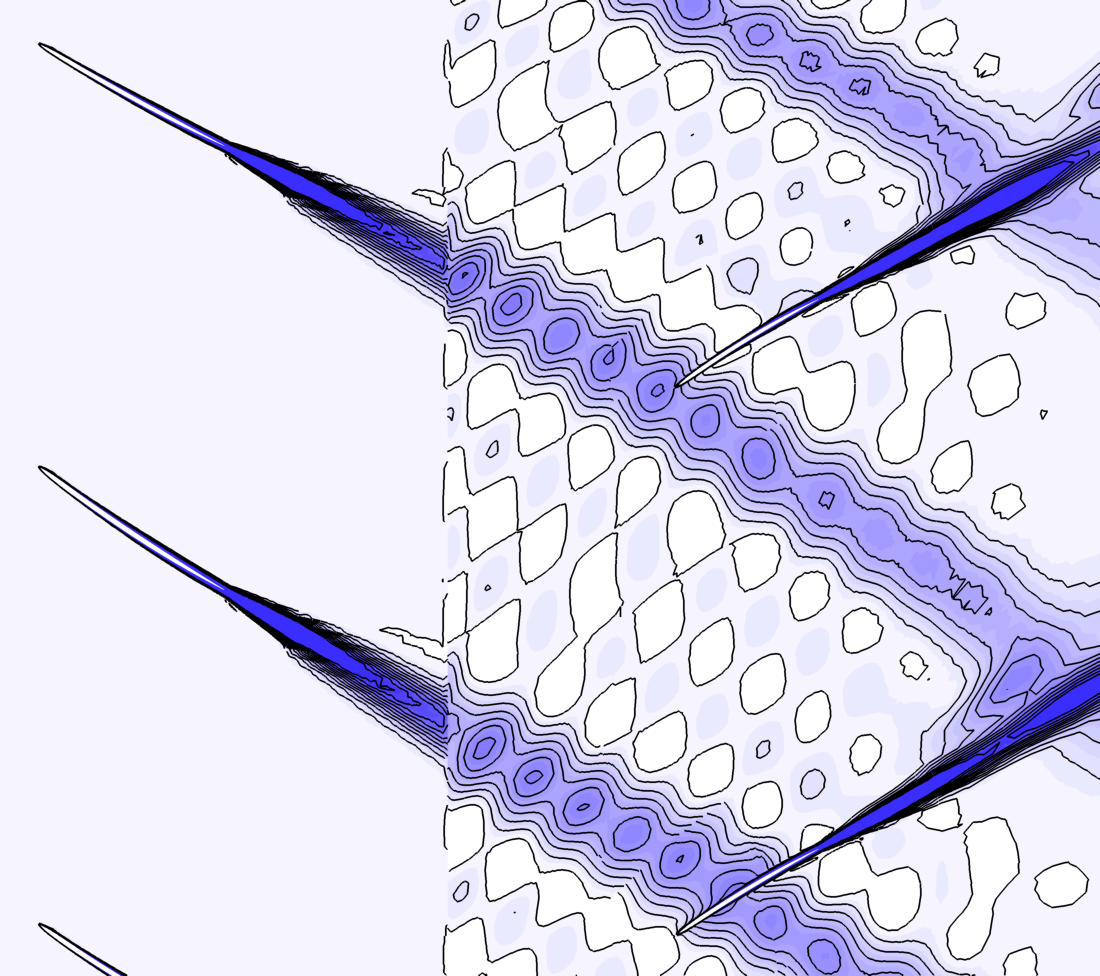
\includegraphics[width=.3\textwidth]{dream_HS_N03_entropy_75.jpg}}
  \subfigure[$N=4$]{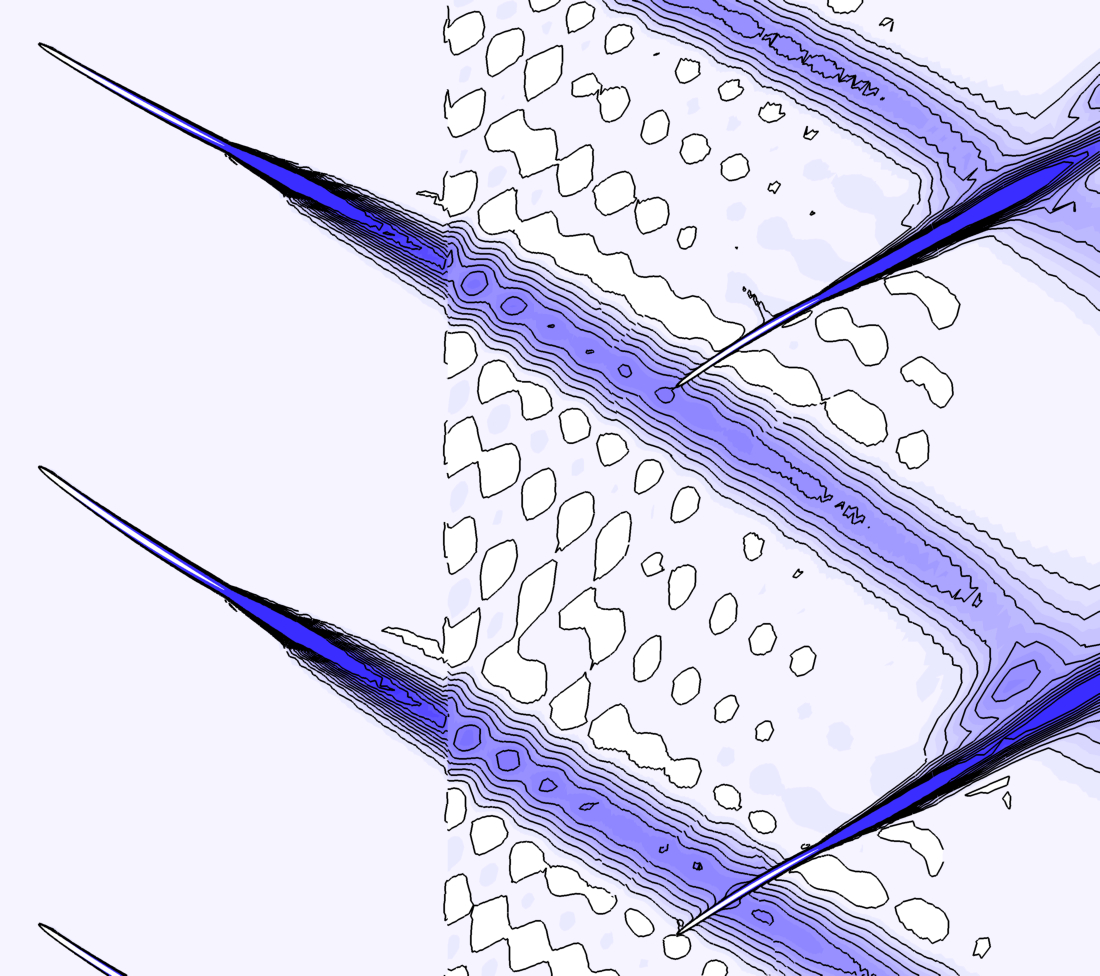
\includegraphics[width=.3\textwidth]{dream_HS_N04_entropy_75.jpg}}
  \subfigure[$N=5$]{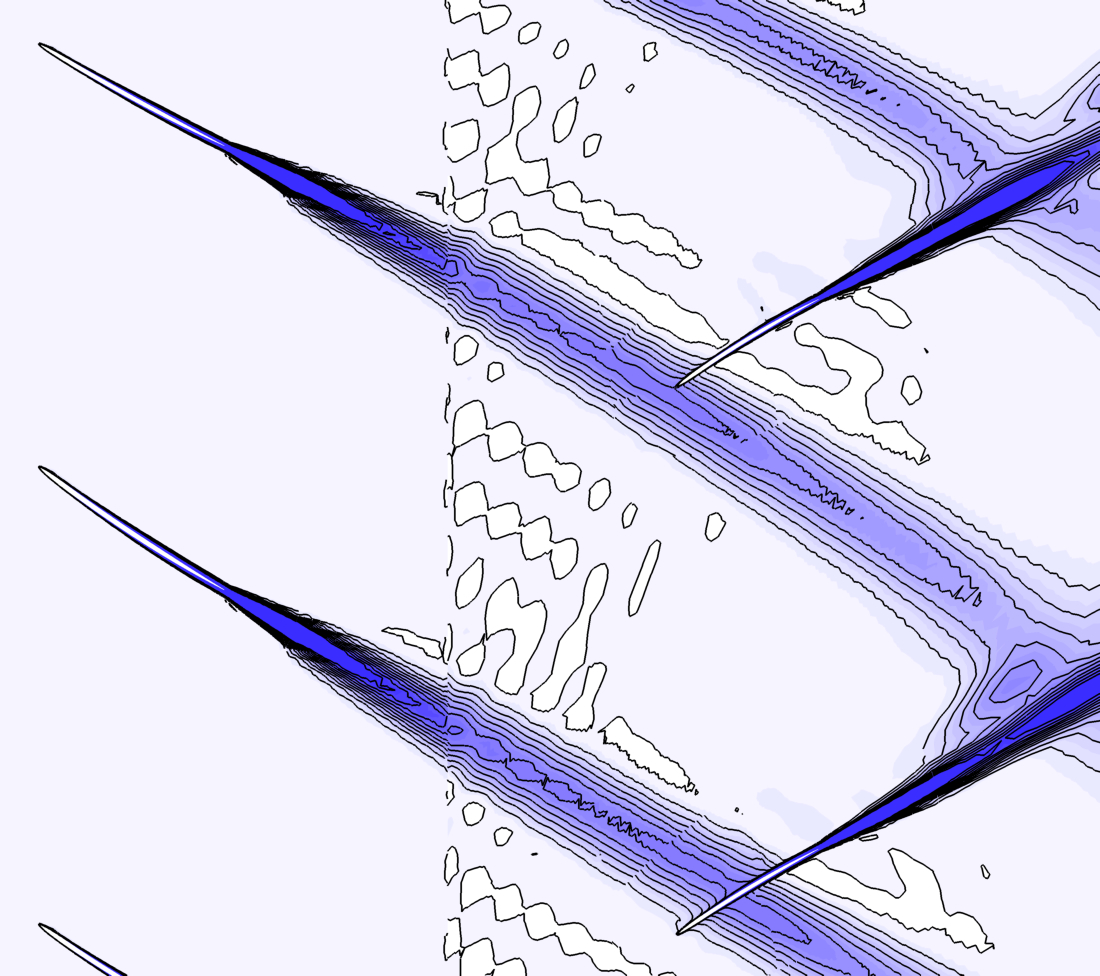
\includegraphics[width=.3\textwidth]{dream_HS_N05_entropy_75.jpg}}
  \subfigure[$N=6$]{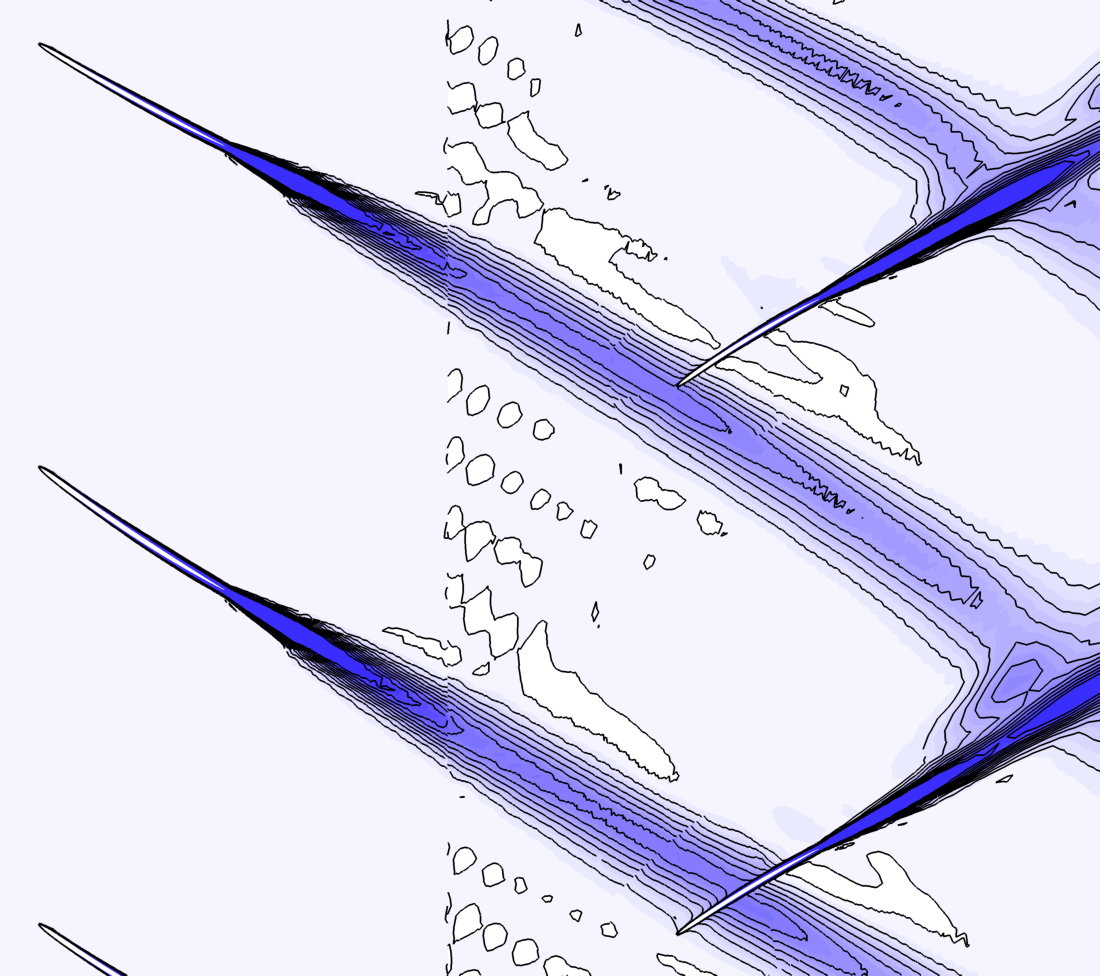
\includegraphics[width=.3\textwidth]{dream_HS_N06_entropy_75.jpg}}
  \subfigure[$N=7$]{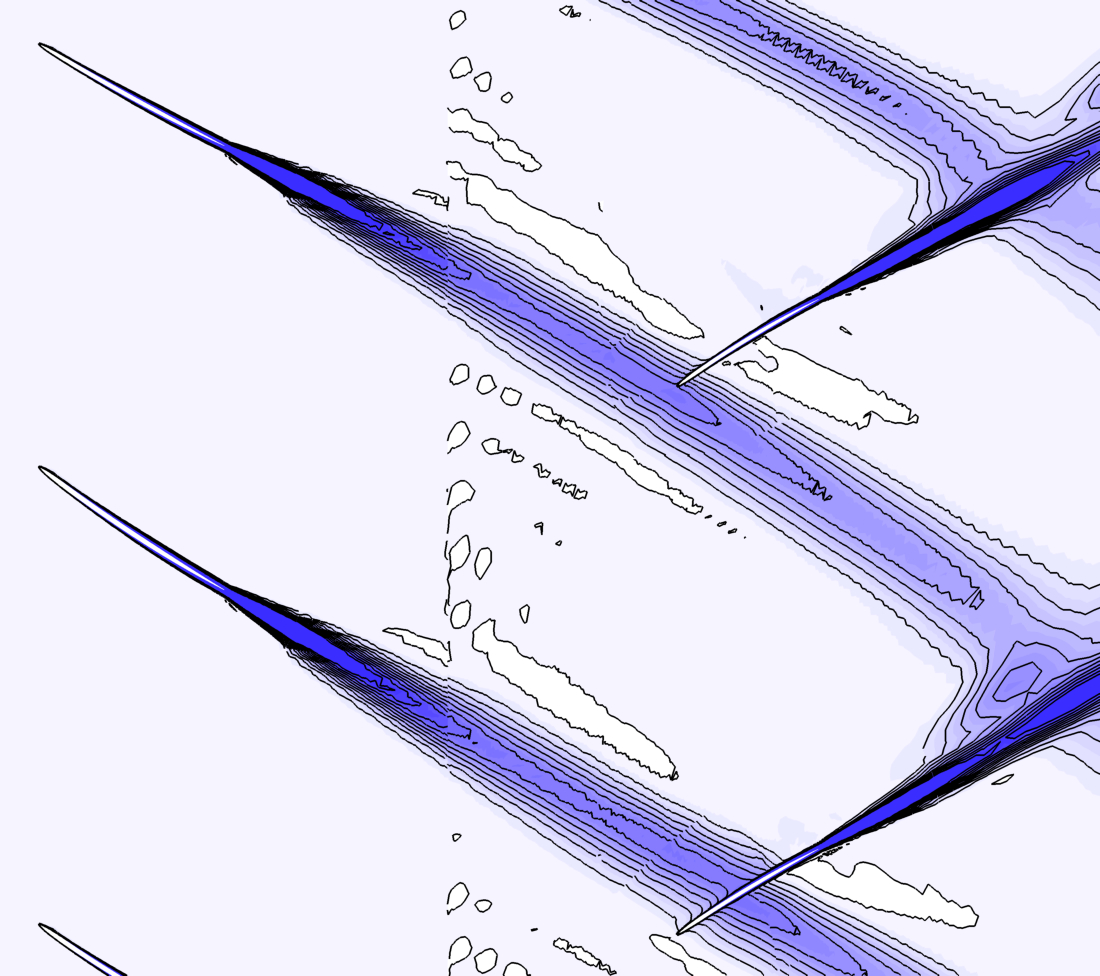
\includegraphics[width=.3\textwidth]{dream_HS_N07_entropy_75.jpg}}
  \subfigure[$N=8$]{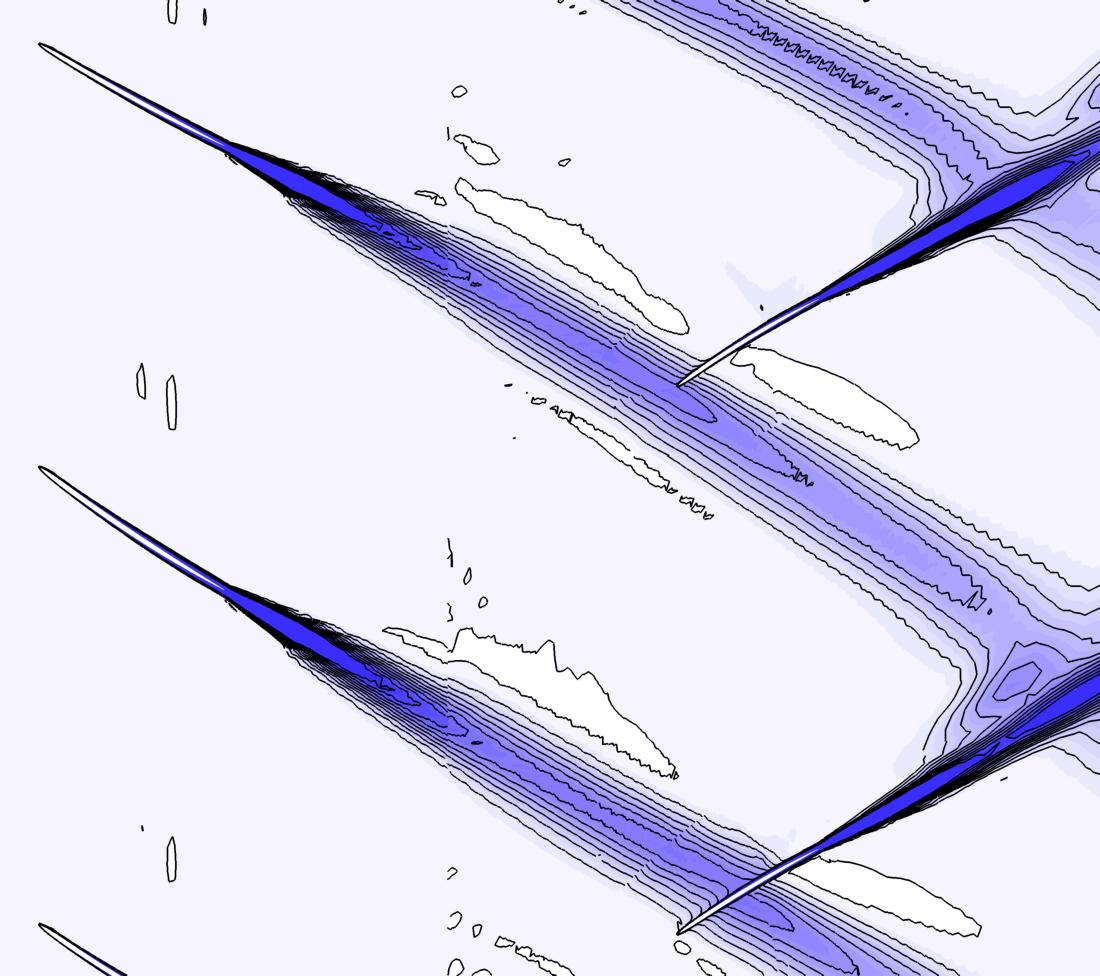
\includegraphics[width=.3\textwidth]{dream_HS_N08_entropy_75.jpg}}
  \subfigure[$N=9$]{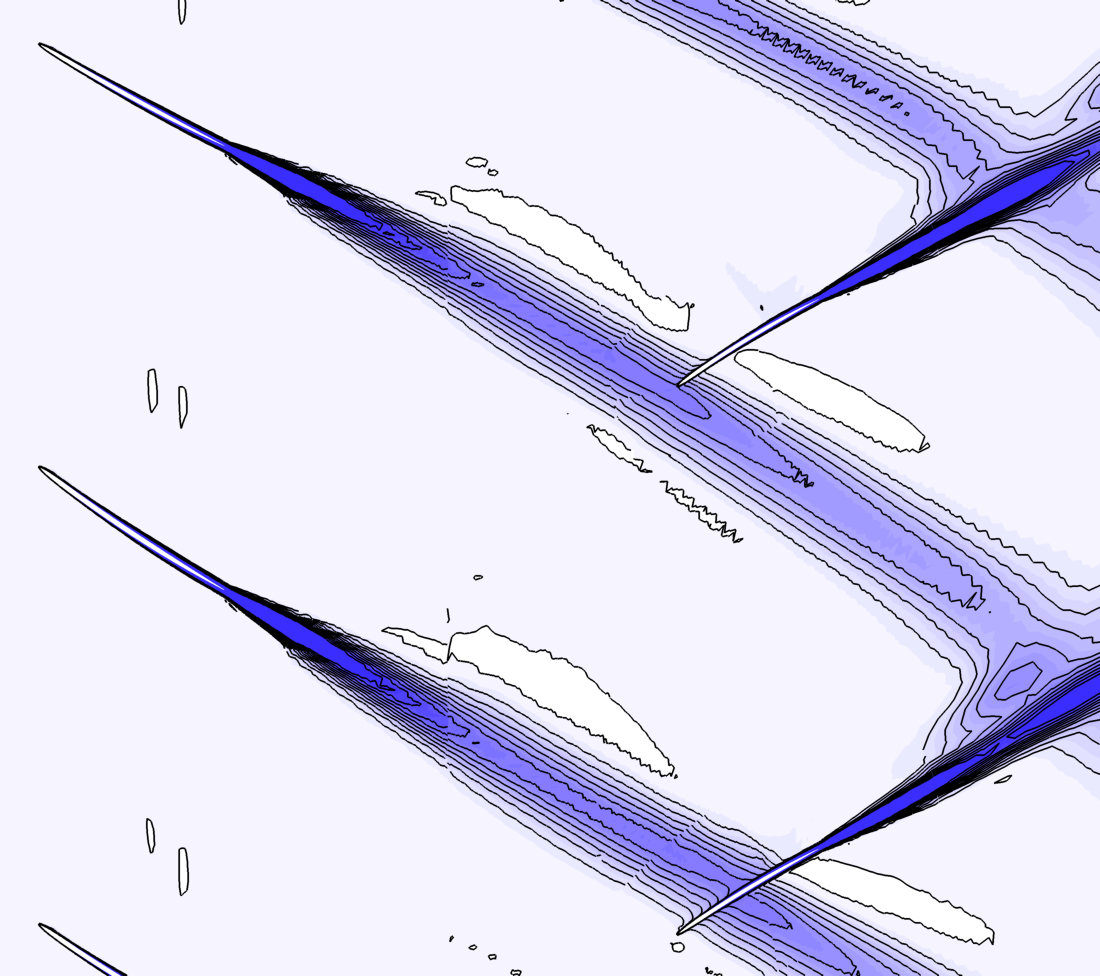
\includegraphics[width=.3\textwidth]{dream_HS_N09_entropy_75.jpg}}
  \caption{\mockup-HS convergence -- Non-dimensional entropy at 75\% span.}
  \label{fig:muhscv}
\end{figure}

For the \aipx configuration, Fig.~\ref{fig:aipx7cv} shows that the convergence is
not achieved as the finest HB computation ($N=10$) still not capture correctly
the wake through the interface. It is thickened by the low time
resolution. Although the solver is
able to account for an arbitrary number of time samples, the required
memory becomes too demanding and only $N=1$ to 10 were attempted. 
\begin{figure}[htp]
  \centering
  \subfigure[$N=1$]{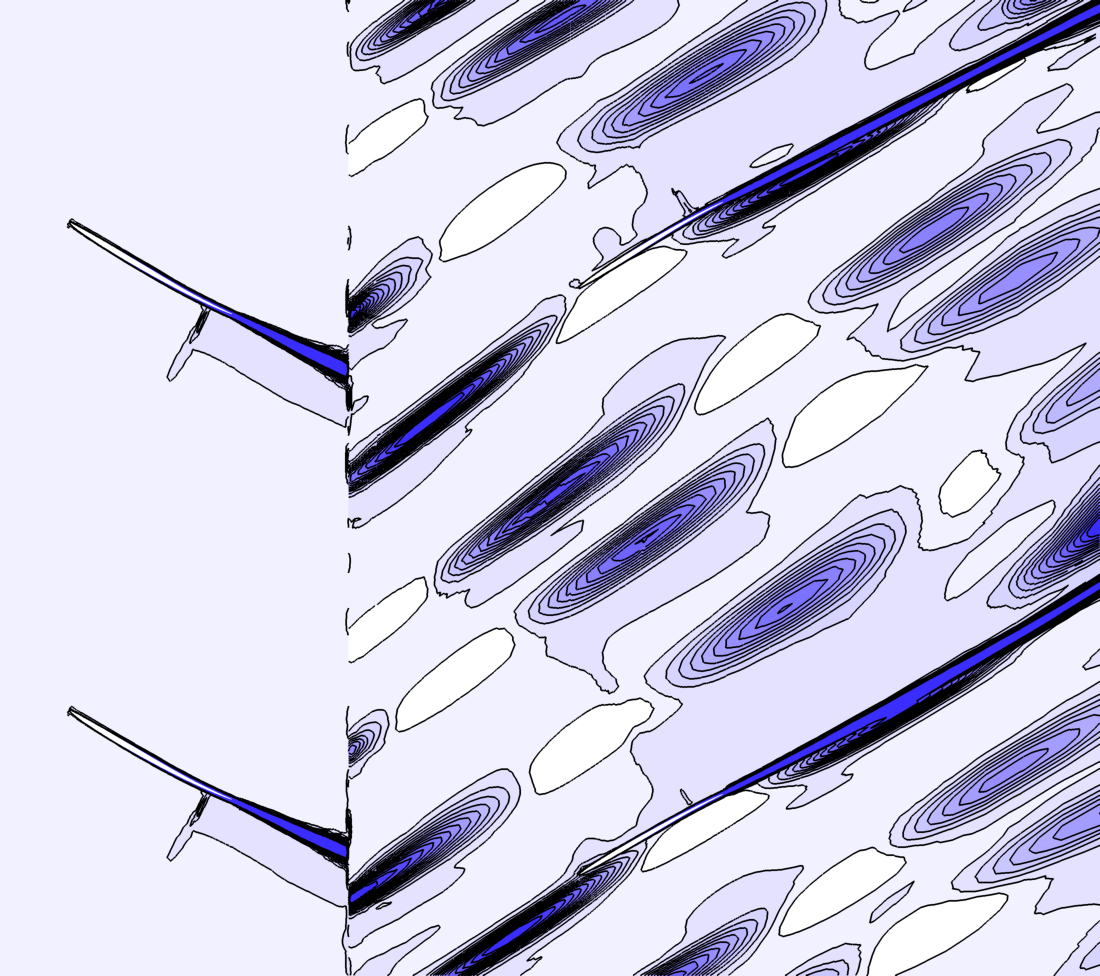
\includegraphics[width=.3\textwidth]{aipx7_N01_entropy_75.jpg}}
  \subfigure[$N=2$]{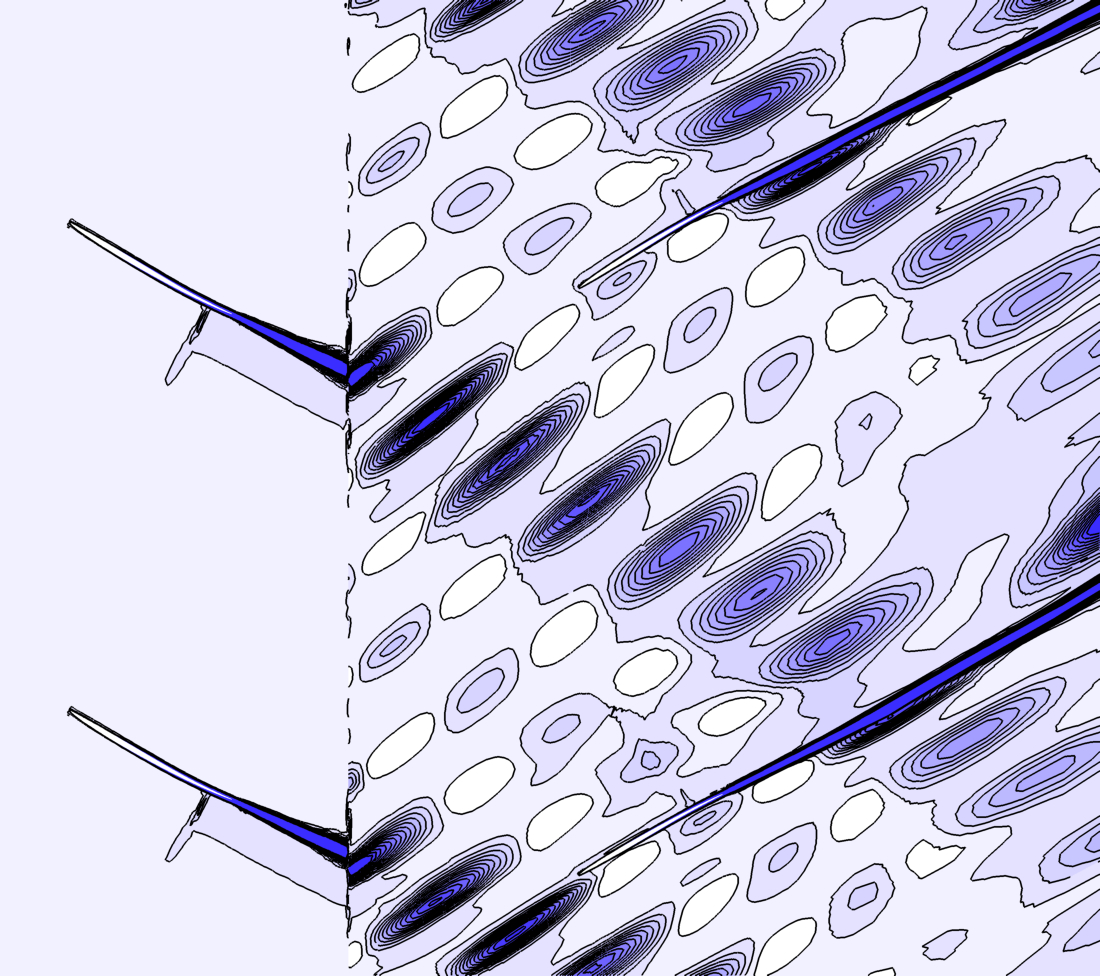
\includegraphics[width=.3\textwidth]{aipx7_N02_entropy_75.jpg}}
  \subfigure[$N=3$]{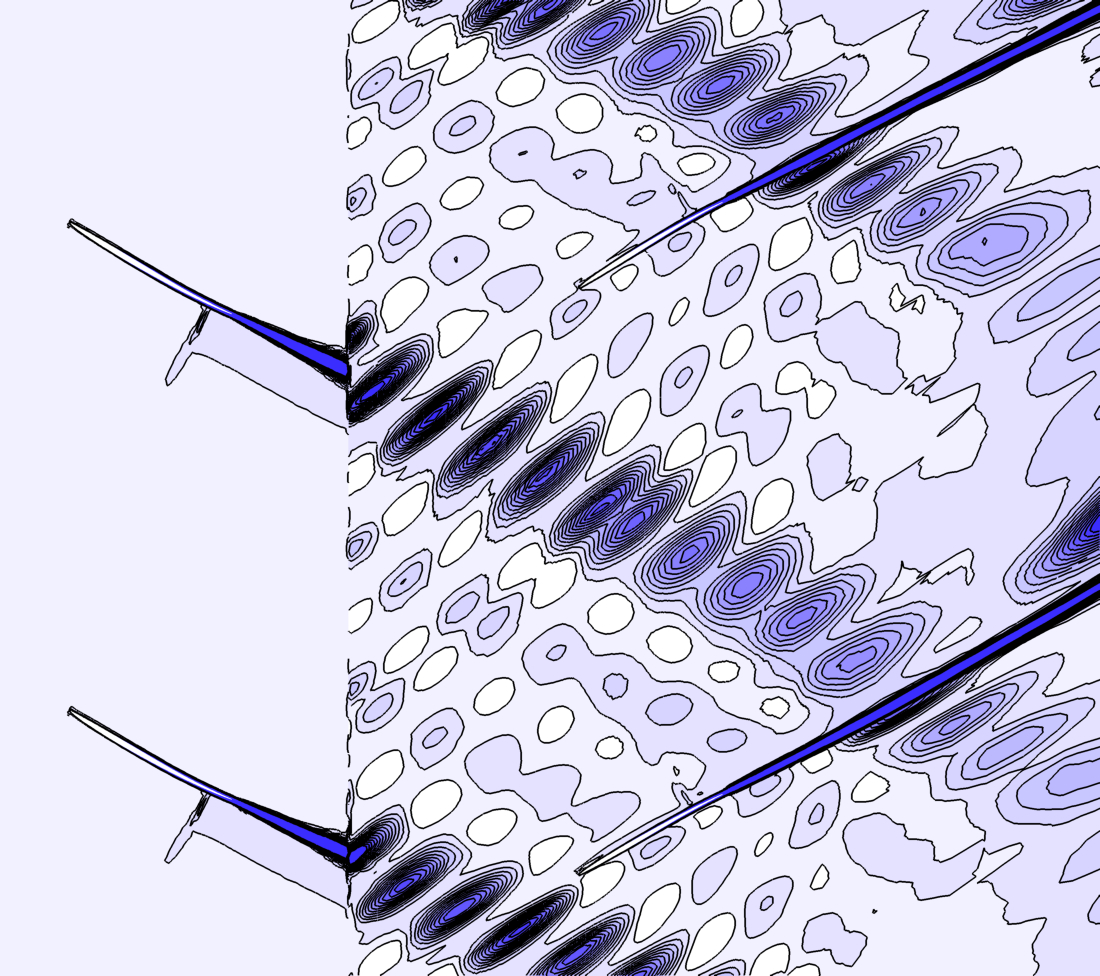
\includegraphics[width=.3\textwidth]{aipx7_N03_entropy_75.jpg}}
  \subfigure[$N=4$]{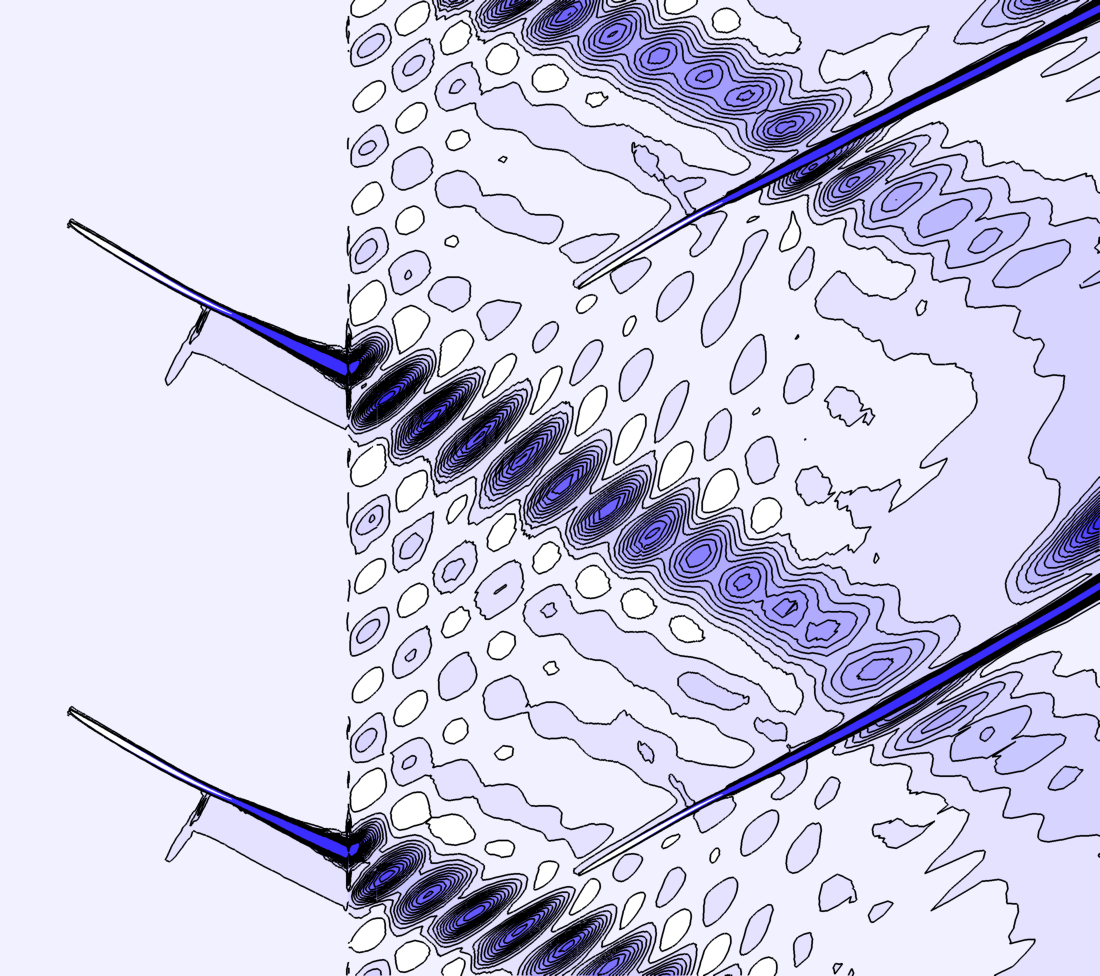
\includegraphics[width=.3\textwidth]{aipx7_N04_entropy_75.jpg}}
  \subfigure[$N=5$]{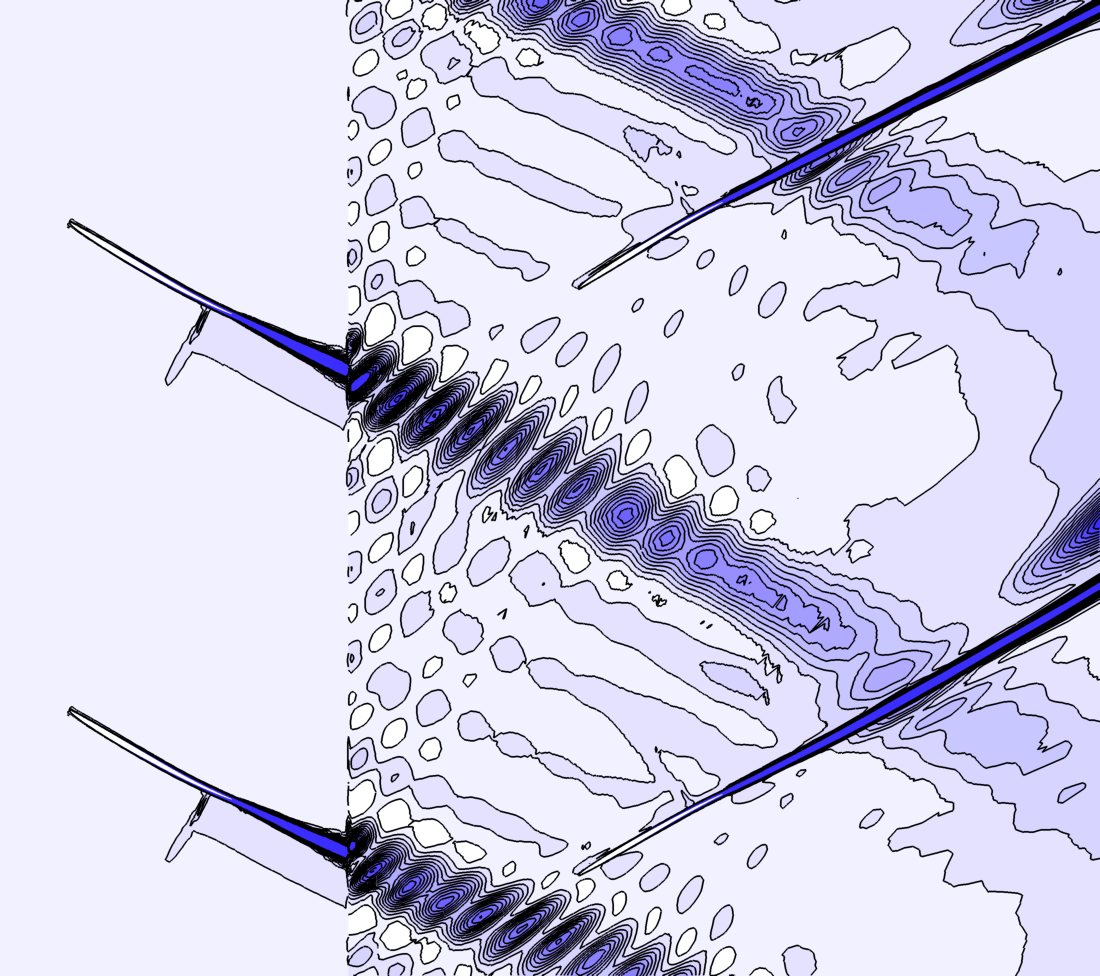
\includegraphics[width=.3\textwidth]{aipx7_N05_entropy_75.jpg}}
  \subfigure[$N=6$]{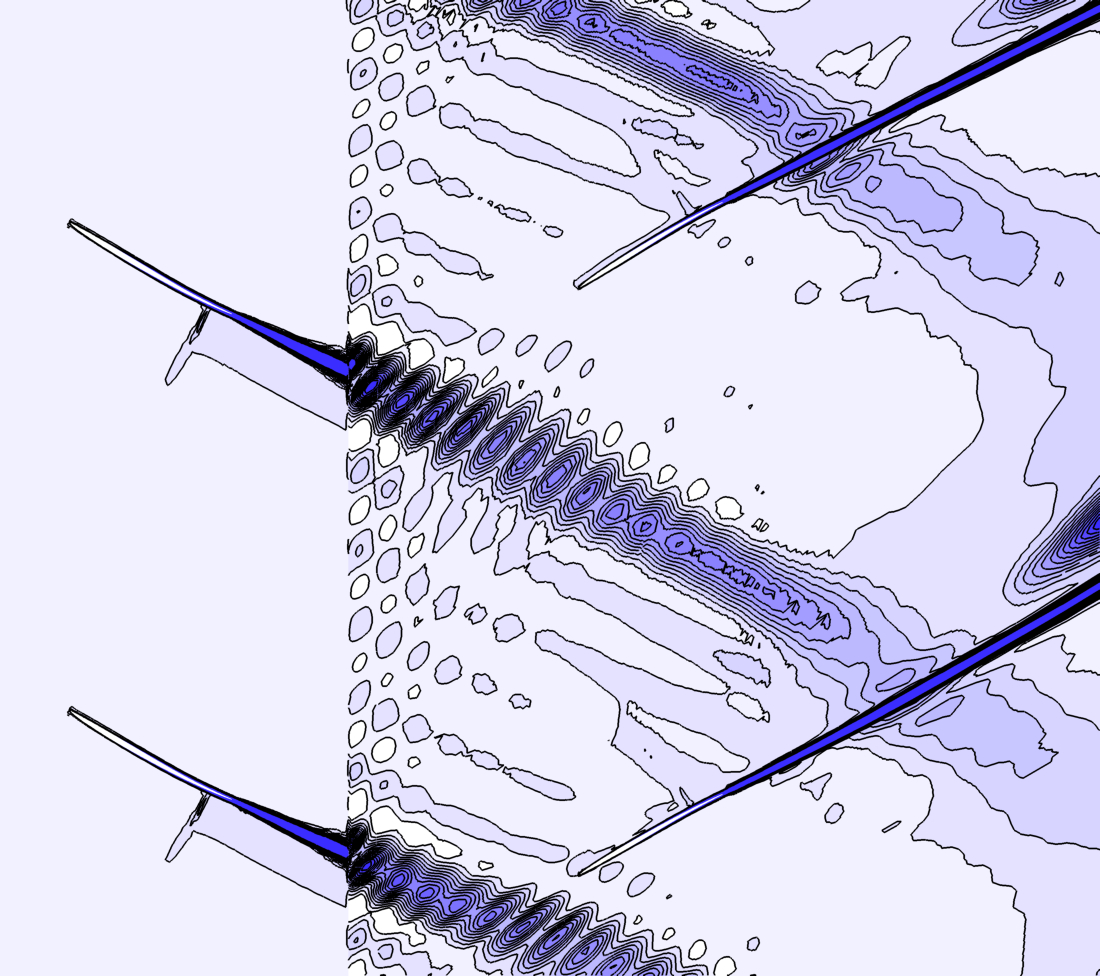
\includegraphics[width=.3\textwidth]{aipx7_N06_entropy_75.jpg}}
  \subfigure[$N=7$]{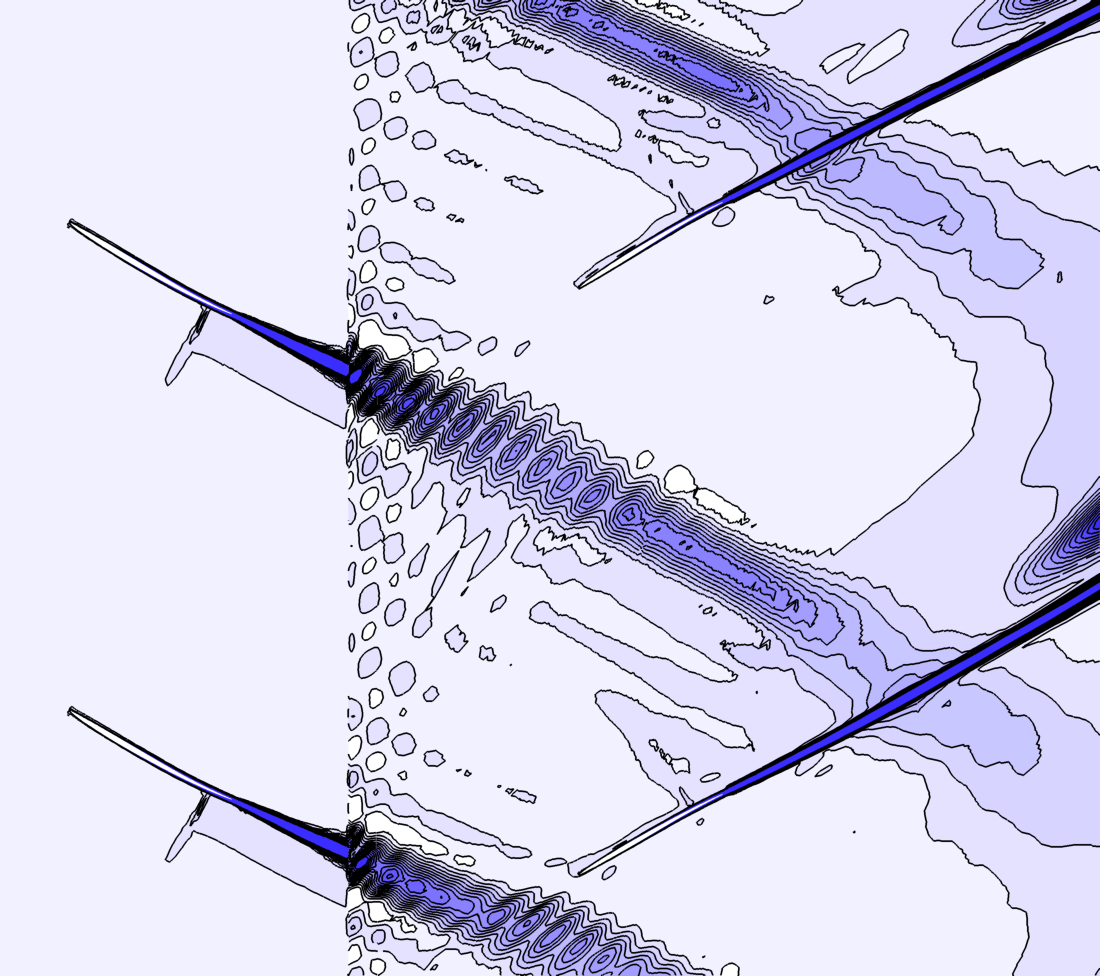
\includegraphics[width=.3\textwidth]{aipx7_N07_entropy_75.jpg}}
  \subfigure[$N=8$]{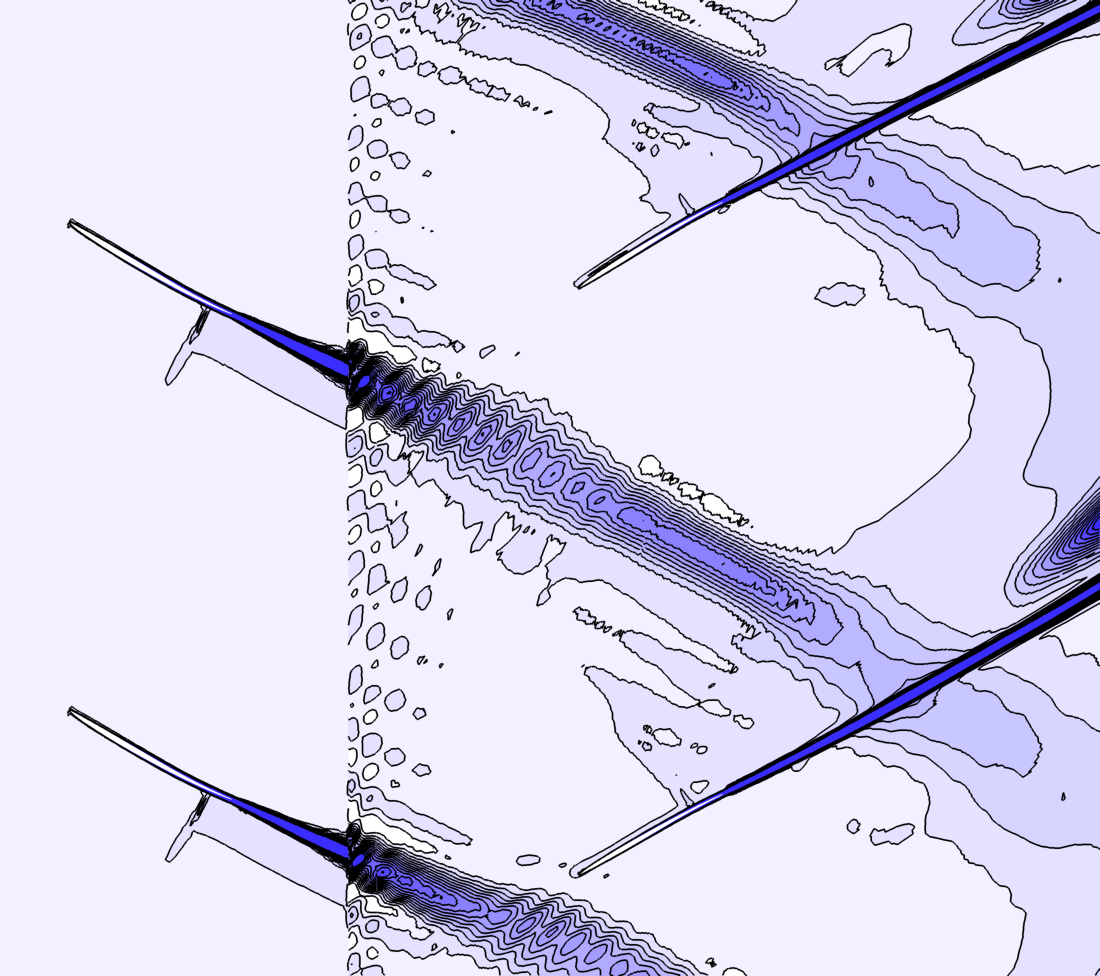
\includegraphics[width=.3\textwidth]{aipx7_N08_entropy_75.jpg}}
  \subfigure[$N=9$]{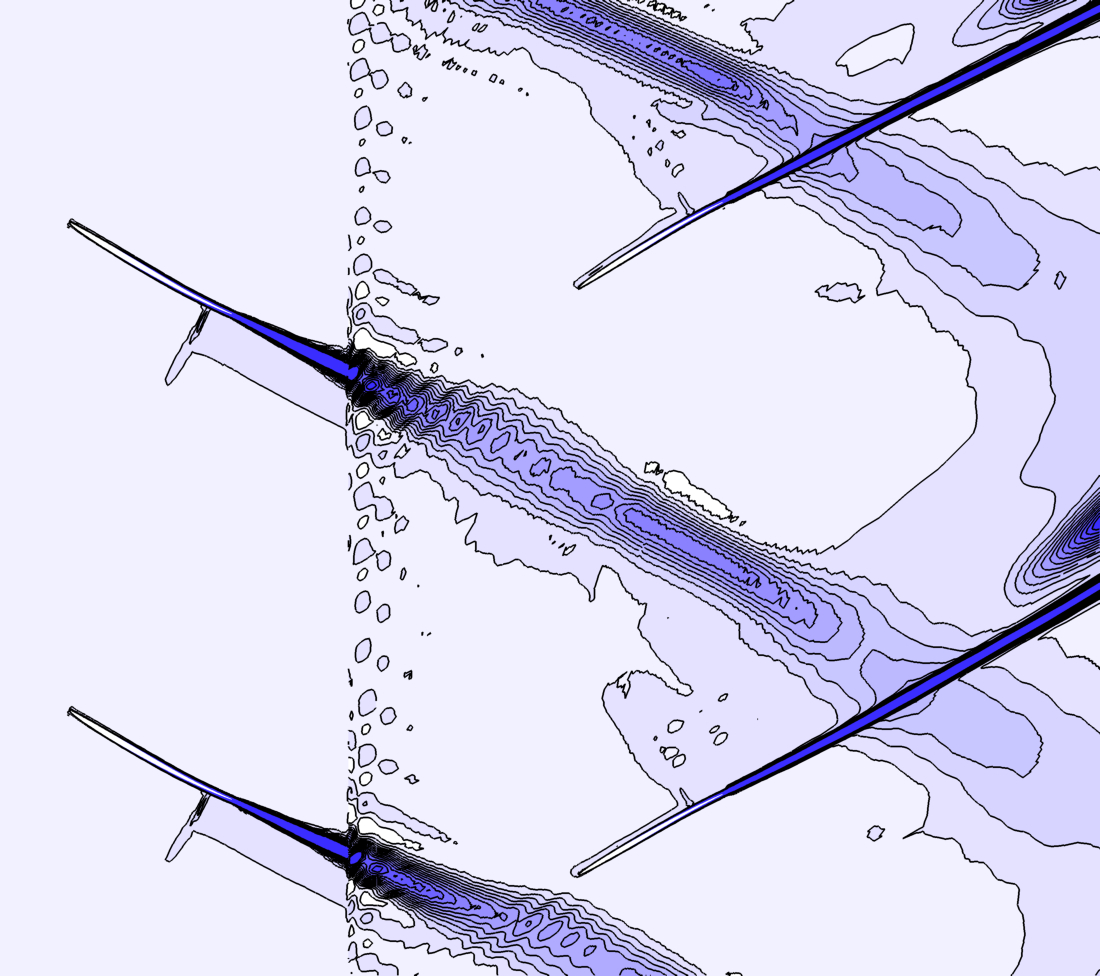
\includegraphics[width=.3\textwidth]{aipx7_N09_entropy_75.jpg}}
  \subfigure[$N=10$]{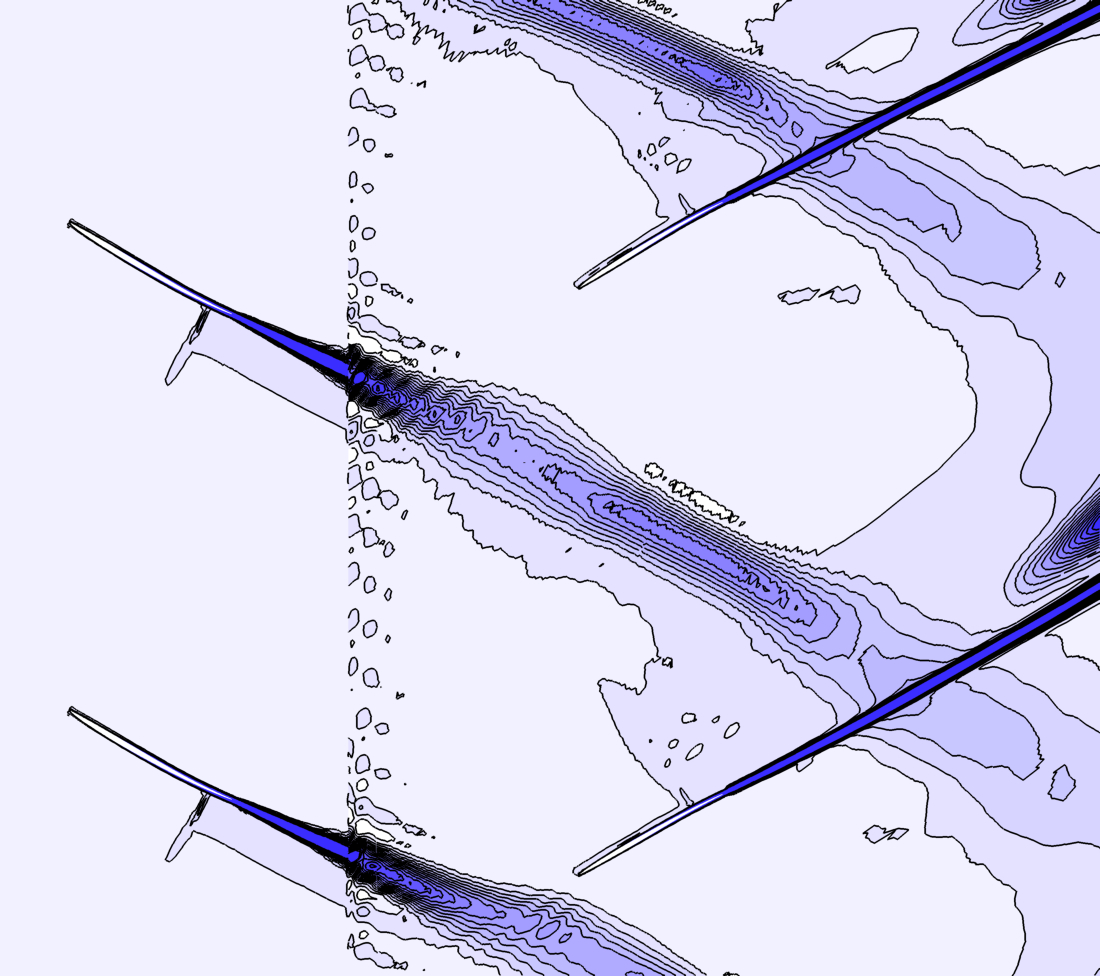
\includegraphics[width=.3\textwidth]{aipx7_N10_entropy_75.jpg}}
  \caption{\aipx-HS convergence -- Non-dimensional entropy at 75\% span.}
  \label{fig:aipx7cv}
\end{figure}

The are two main differences with the \mockup-HS configuration:
\begin{enumerate}
\item the \aipx configuration is at scale meaning the radial extent is
  several times larger than the \mockup configuration. As the
  pitchwise relative wake width is defined as
  \begin{equation}
    L_{pitch}=L\frac{B}{2\pi R},
  \end{equation}
  the relative wake width will decrease for higher radius~$R$. It also
  explains the difference with classical turbomachinery: as the number
  of blades $B$ can be one order of magnitude higher in the latter
  case than in a CROR configuration and the diameter lower, the
  relative wake thicknesses are higher and the spectrum narrower.
\item the viscosity is also different: applying the Sutherland law for
  air at ground and flight level leads to dynamic viscosities of,
  respectively, $1.807\cdot 10^{-5}$~Pa.s and $1.434\cdot
  10^{-5}$~Pa.s. With lower viscosity, the blade boundary layer is
  thinner and the generated wakes are thinner as well. Furthermore,
  the mixing with the main flow is weaker and the thickening of the
  wakes is also slower leading to a thinner wake reaching the blade
  row interface.
\end{enumerate}

\FloatBarrier

\subsection{Prediction tool based on the wake thickness}
To estimate the wake thickness, a curve fitting algorithm is used to
fit the CFD wakes to the Lakshminarayana and Davino Gaussian wake
law.
Only the relative span between 10\% and 70\% is
considered as elsewhere, the wake interacts with the hub boundary layer and
tip vortex.  This
estimation is plotted in Fig.~\ref{fig:crorwakethick} for the three
configurations.
\begin{figure}[htp]
  \centering
  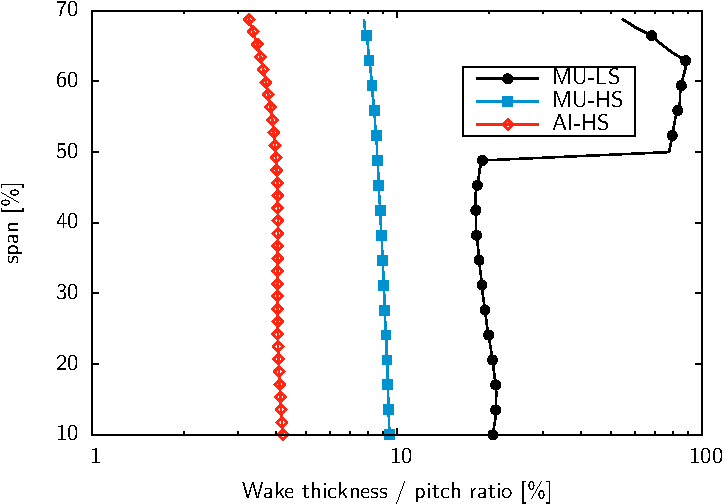
\includegraphics[width=.45\textwidth]{CROR_THICKNESS.pdf}
  \caption{Estimation of the relative wake thickness for the three contra-rotating
  open rotor configurations.}
  \label{fig:crorwakethick}
\end{figure}
The wake thickness is almost constant along the span for the two HS configurations.
In opposite, the \mockup-LS shows an increase at 50\% of the
relative span. This is due to a large tangential distortion that is
attributed to  flow separation. Thus, the wake width estimation
is not reliable in this region for the \mockup-LS configuration as the
tangential distortion is no longer Gaussian-shaped.
Nevertheless, using Fig.~\ref{fig:crorwakethick}, the wake widths
of the \aipx-HS, the \mockup-HS and the \mockup-LS are approximately
4\%, 9.5\% and 20\%, respectively. 

The level of accumulated energy required 
for a computation to be rigorously converged
is difficult to estimate. 
It seems reasonable, from an engineering standpoint, to consider
that a 99\% accumulation of energy should be a good criterion.
To emphasize that,
the reconstruction of a wake as a function of four levels of cumulative
energy $E$ is depicted in Fig.~\ref{fig:level_of_energy}. 
\begin{figure}[htp]
  \centering
  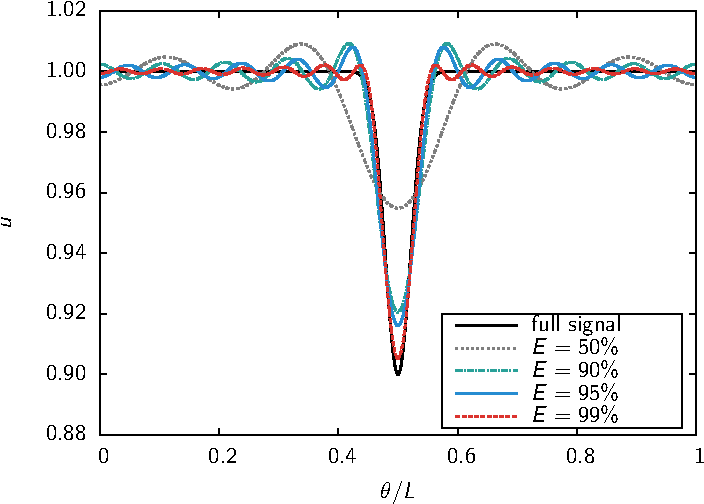
\includegraphics[width=.5\textwidth]{LEVEL_OF_ENERGY_PAPER.pdf}
  \caption{Reconstructions of a wake depending on
  the energy content kept in the signal.}
  \label{fig:level_of_energy}
\end{figure}
One can see
that a reconstruction using only 50\% of the energy
leads to a signal that has neither
the right wake deficit nor the correct width. Using
90\% and 95\% of the energy improve the resulting shape
but  large secondary
oscillations remain, with a bad capture
of the wake deficit.
In opposite, by using 99\% of the energy to reconstruct
the signal, only minor
oscillations are seen but 
the wake width and deficit are recovered with more than 
95\% accuracy.
Thus, the 99\% energy threshold ensures that the wake
will be correctly transmitted to the opposite row, which is
the prior concern of this paper.
Therefore, based on this value
and the estimation of the wake width
for all the three CROR configurations shown in Fig.~\ref{fig:crorwakethick},
one can evaluate the number of harmonics needed to compute such
applications.
In fact, based on the
analytic formula derived in Sec.~\ref{sec:turbomachine_wake}
and the equivalence of truncation error and accumulated energy given by
Eq.~\eqref{eq:correspond_E_error},
if the wake width is known, one can deduce the
number of harmonics~$N$ needed to capture a target level of accumulated energy
$E$:
\begin{equation}
    N(E) = \frac{\erfc^{-1} \left[1 - E \right]}{
    \sqrt{2 \alpha^\prime}},
    \label{eq:estimation_nb_harms}
\end{equation}
where $\alpha^\prime$ is
the wake parameter as defined in 
Sec.~\ref{sec:turbomachine_wake}:
\begin{equation}
    \alpha^\prime(L) =  \frac{1}{0.693} \left( \frac{\pi L}{2} \right)^2.
\end{equation}
Here, the theoretical estimation of the number of harmonics needed 
to recover 99\% of the energy is then
17, 7 and 3 for, respectively, the \aipx-HS, the \mockup-HS
and the \mockup-LS. These numbers explain why the 
\aipx-HS configuration is still not converged after $N=10$
harmonics. In fact, such a computation leads to recover only
87\% of the signal energy. Figure~\ref{fig:level_of_energy}
supports the argument that with this level of energy, the wake
is not properly captured as a 90\% energy signal
does not accurately estimate the wake deficit and thickness.

With this approach, one can deduce approximately
the number of harmonics needed to compute such CROR
configurations using Fourier-based time methods for a target level
of accumulated energy. The issue is that it is limited to
Gaussian wakes. If the wake shape is very different from a Gaussian
curve or if another tangential
distortion reaches the interface, the present
prediction tool cannot be used. 
However, as demonstrated in Sec.~\ref{sub:comp_w_analytic},
the analytic error and the error based on an
azimuthal Fourier transform of the distortion
seen just upstream the interface for a mixing-plane
configuration are equivalent. 


\subsection{Prediction tool based on an azimuthal Fourier transform}
\label{sub:prediction_tool_azimuthal_fft}
Thus, a more general way to analyze the spectrum in a wake is
to perform an azimuthal Fourier transform at the rows interface
in a mixing-plane computation. It encompasses both the wake analysis done above and also
any tangential disturbances, as for instance
the viscosity effects near the hub or the tip vortex.
Details of the algorithm used to compute the tangential accumulated
energy from a mixing plane computation are given in \ref{app:epsilon_cror_steps}.

To have a global insight of the energy contained in the
tangential distortion across the whole span,
the energy accumulation is plotted using a color map
in Fig.~\ref{fig:crorroxvmapenergy}.
Three contour lines are added to ease the
interpretation: 90\%, 95\%
and 99\% of accumulated energy, corresponding to a truncation
error of respectively 30\%, 20\% and 10\%.
\begin{figure}[htp]
  \centering
  \subfigure[\mockup-LS]{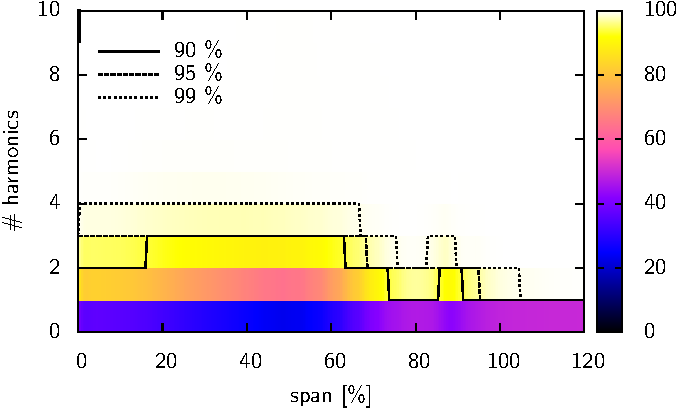
\includegraphics[width=.46\textwidth]{DREAM_LS_RANS_ROE2_SPECTRUM_PPT.pdf}}
  \subfigure[\mockup-HS]{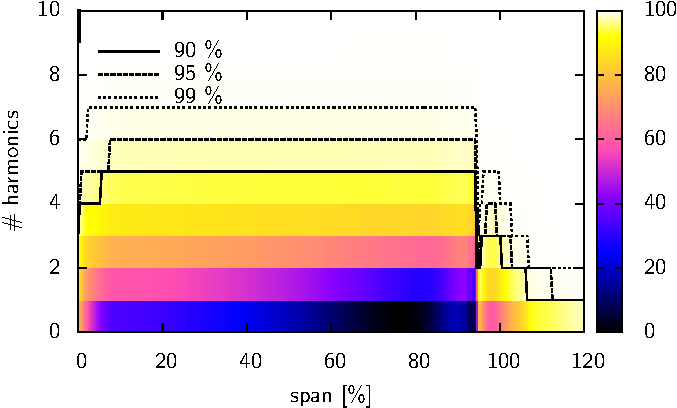
\includegraphics[width=.46\textwidth]{DREAM_HS_RANS_ROE2_SPECTRUM_PPT.pdf}}
  \subfigure[\aipx-HS]{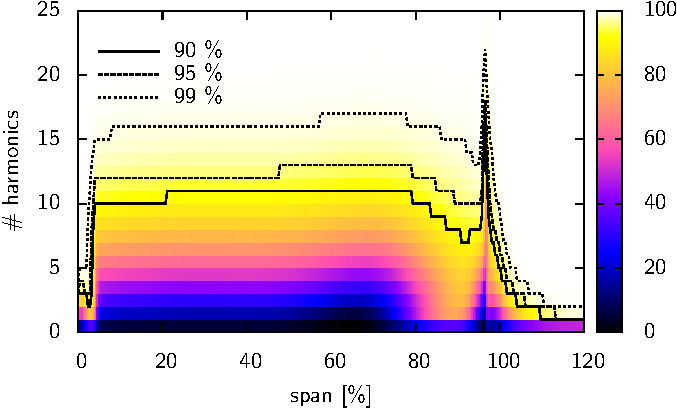
\includegraphics[width=.46\textwidth]{AIPX7_RANS_SPECTRUM_PPT.pdf}}
  \caption{Energy accumulation by harmonics for all spans.}
  \label{fig:crorroxvmapenergy}
\end{figure}
The richer spectrum is observed 
in the wake region between
10\% and 70\% of relative span. This is the region where the wake is
influenced neither by the hub boundary layer nor by the tip
vortex. Therefore the wake drives 
the convergence of HB computations.
Results are in good agreement with the prediction tool
based on the wake thickness. To emphasize that, the number of harmonics
needed to have 99\% of the energy is given in 
Tab.~\ref{tab:predicted_N_CROR} for a relative
span between 10\% and 70\%.
\begin{table}
  \ra{1.3} 
  \centering
  \begin{tabular}{l|ccc}
    \toprule
    configuration & \aipx-HS & \mockup-HS & \mockup-LS \\
    \midrule
    wake thickness & 17 & 7 & 3 \\
    azimuthal Fourier transform & 16 & 7 & 4 \\
    \bottomrule
  \end{tabular}
\caption{Predicted number of harmonics associated to $E = 99\%$ of 
accumulated energy, using two prediction tools,
the first based on the wake thickness and the second based on
an azimuthal Fourier transform.}
\label{tab:predicted_N_CROR}
\end{table}


This prediction tool is more accurate as it handles
wake tangential distortion as well as any other
type of azimuthal distortions. 
Thus, it can be used to predict
the number of harmonics needed to capture a certain
level of energy for any relative span.
The computational time needed to
get the accumulated energy pictures as in
Fig.~\ref{fig:crorroxvmapenergy} is negligible. In fact, it takes less
than a minute.

We verify \emph{a posteriori} that the number of harmonics
provided in Tab.~\ref{tab:predicted_N_CROR} are sufficient
to yield converged HB computations. For the \mockup-LS, the prediction tool
estimate that four harmonics are sufficient. In fact, Fig.~\ref{fig:mulscv}
supports the argument that four harmonics gives a converged simulation as
the difference between $N=4$, $N=5$ and $N=6$ HB computations are barely
visible. For the \mockup-HS, seven harmonics are estimated to be sufficient
while visually, it seems that $N=8$ is converged. 
In fact, one must keep in mind that these criteria just give a lower
bound of the required number of harmonics needed to get the
convergence of the HB method. Indeed, when running a $N$-harmonic HB
computation, the time period is sampled with $2N+1$ time instants
which is, according to the \citet{Nyquist1928}
criteria,
the minimum sampling to get the $N$\textsuperscript{th} of the
fundamental frequency. It does not necessarily mean that the level of
the $N$\textsuperscript{th} harmonic is accurately
predicted. Experience shows that in order to reach this level, one has
to run a $N+1$ or $N+2$ HB computation. 

Figure~\ref{fig:crorroxvmap} shows the non-dimensional
axial momentum extracted at the rotor/rotor interface
from a single-passage mixing-plane computation
for the three considered configurations.
One can observe different wake shapes: the \aipx High-Speed (HS) wake looks much
thinner than the \mockup-HS, which looks
thinner than the Low-Speed (LS) one. Indeed, the latter does not show a
well delimited wake structure all along the span explaining the estimation of the
number of harmonics needed to capture such configurations.
\begin{figure}[htp]
  \centering
  \subfigure[\mockup-LS]{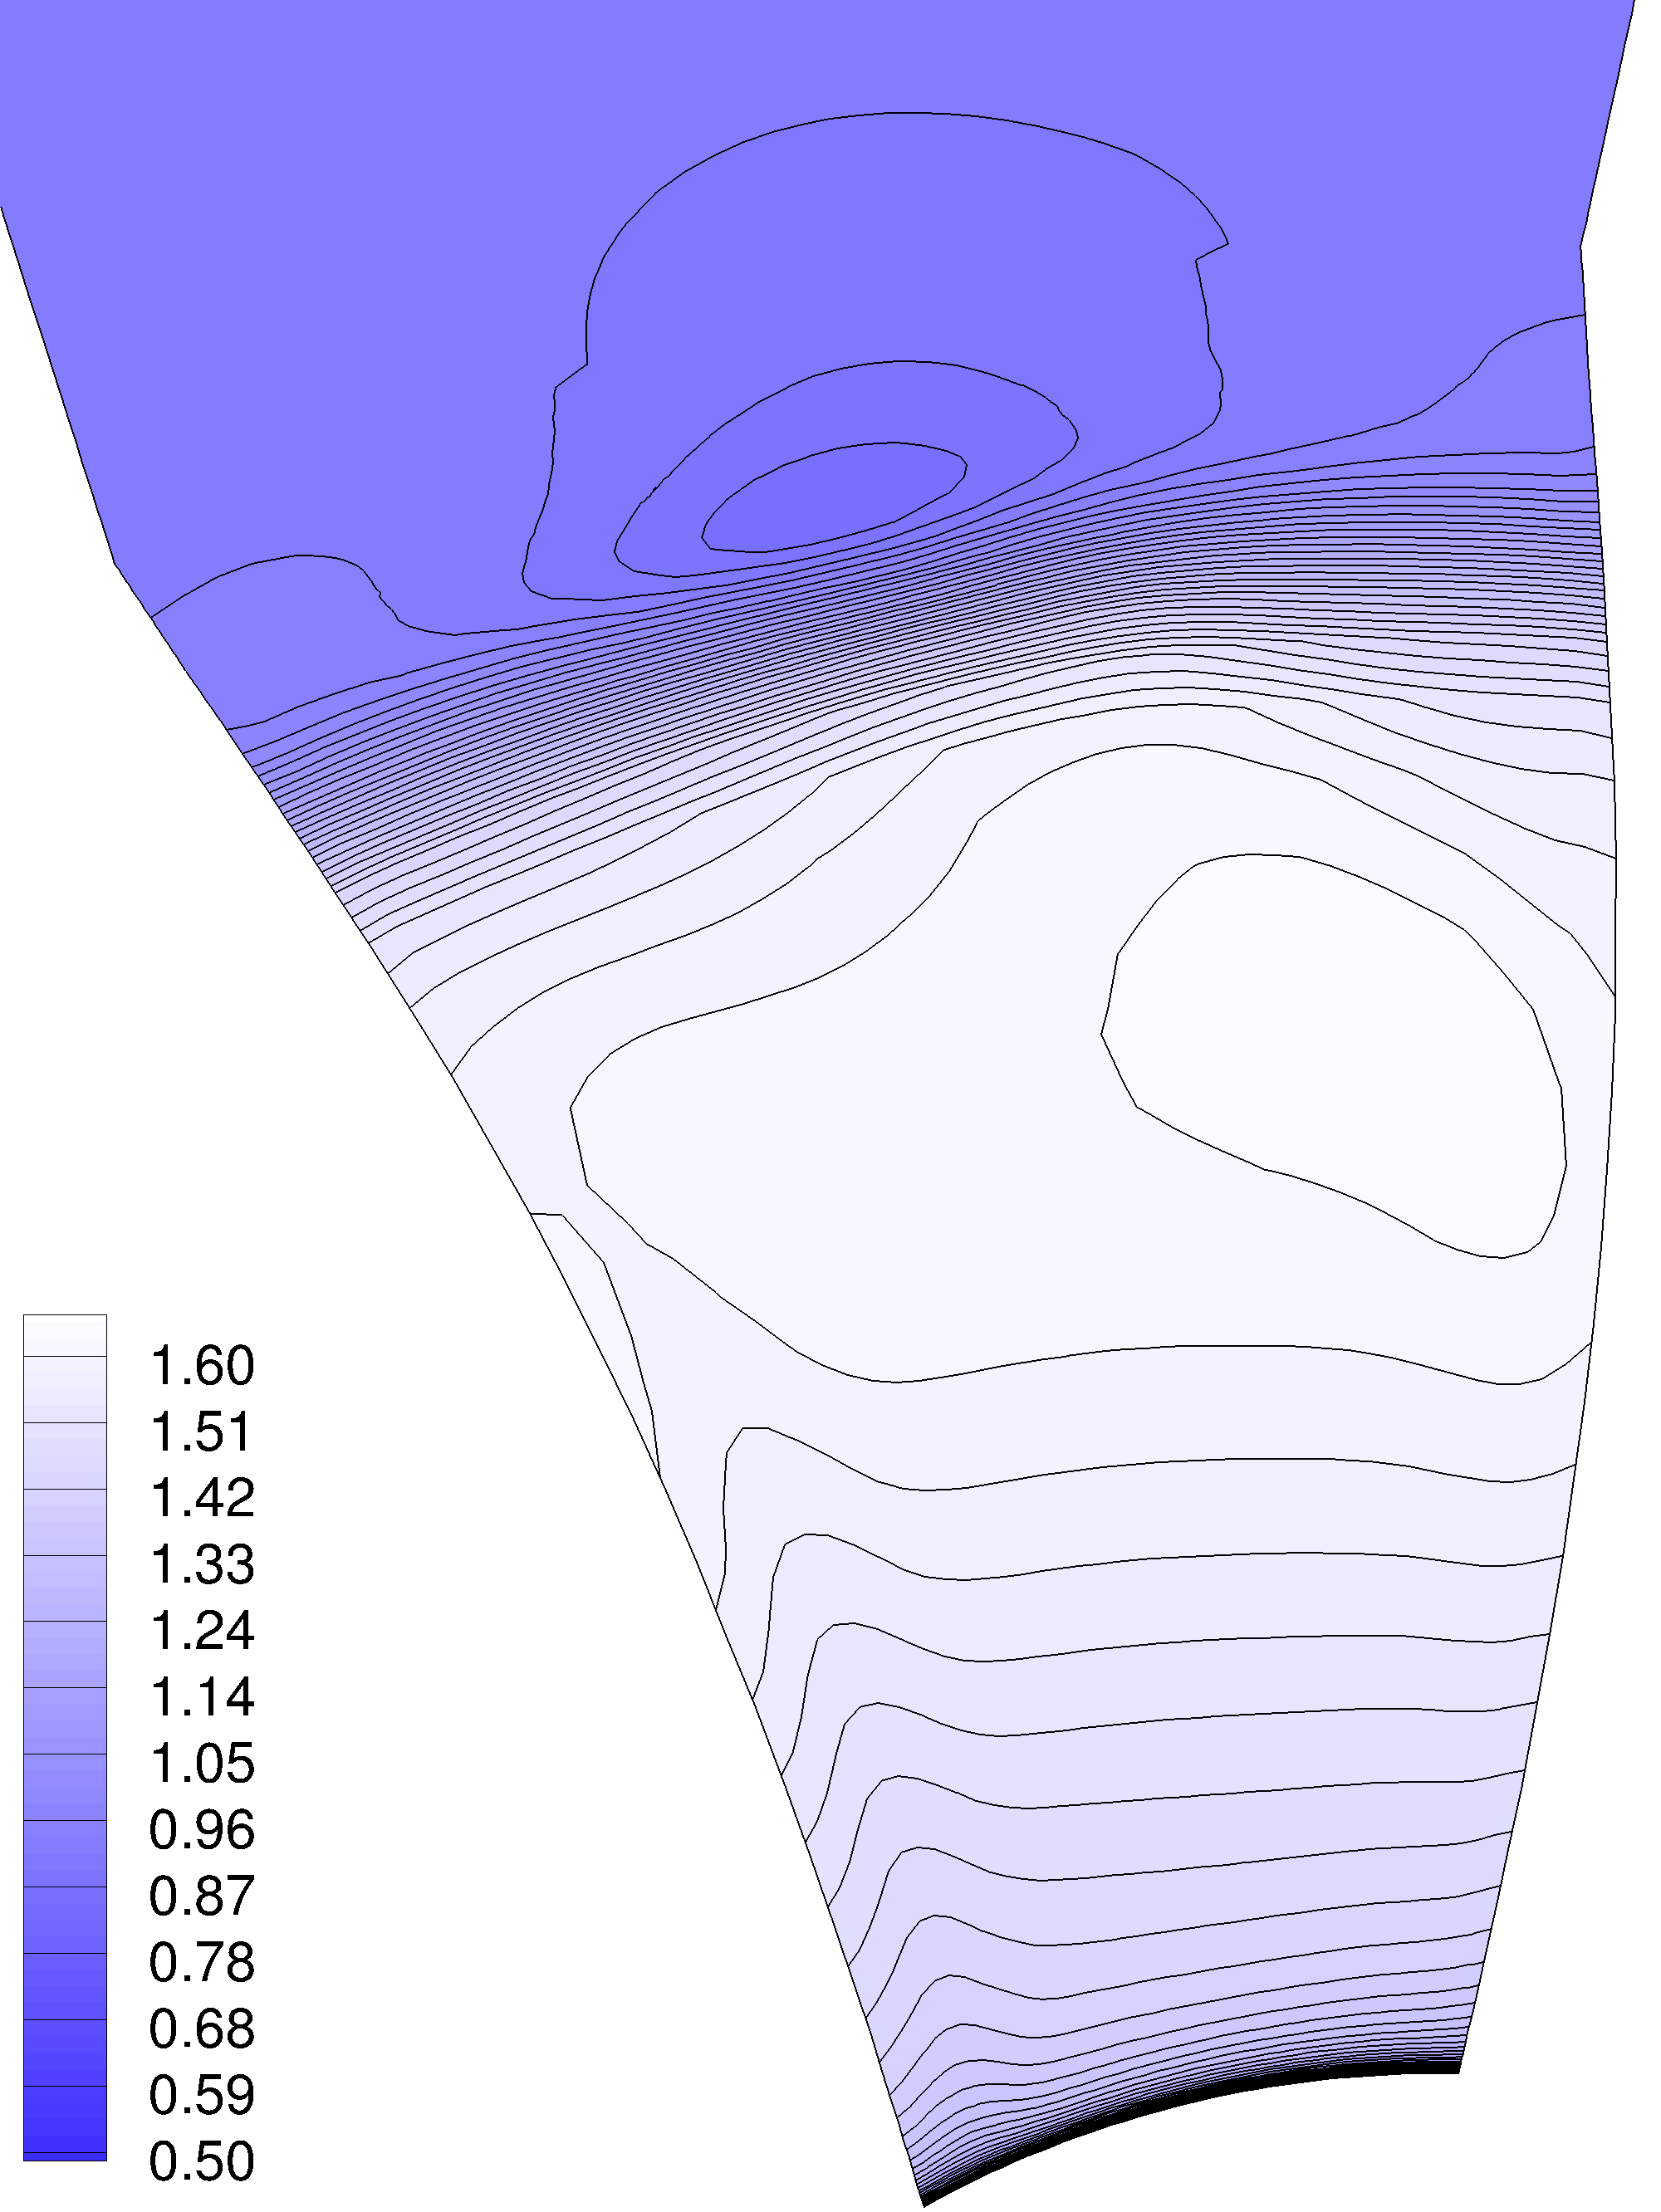
\includegraphics[width=.2\textwidth]{dream_ls.png}}
  \subfigure[\mockup-HS]{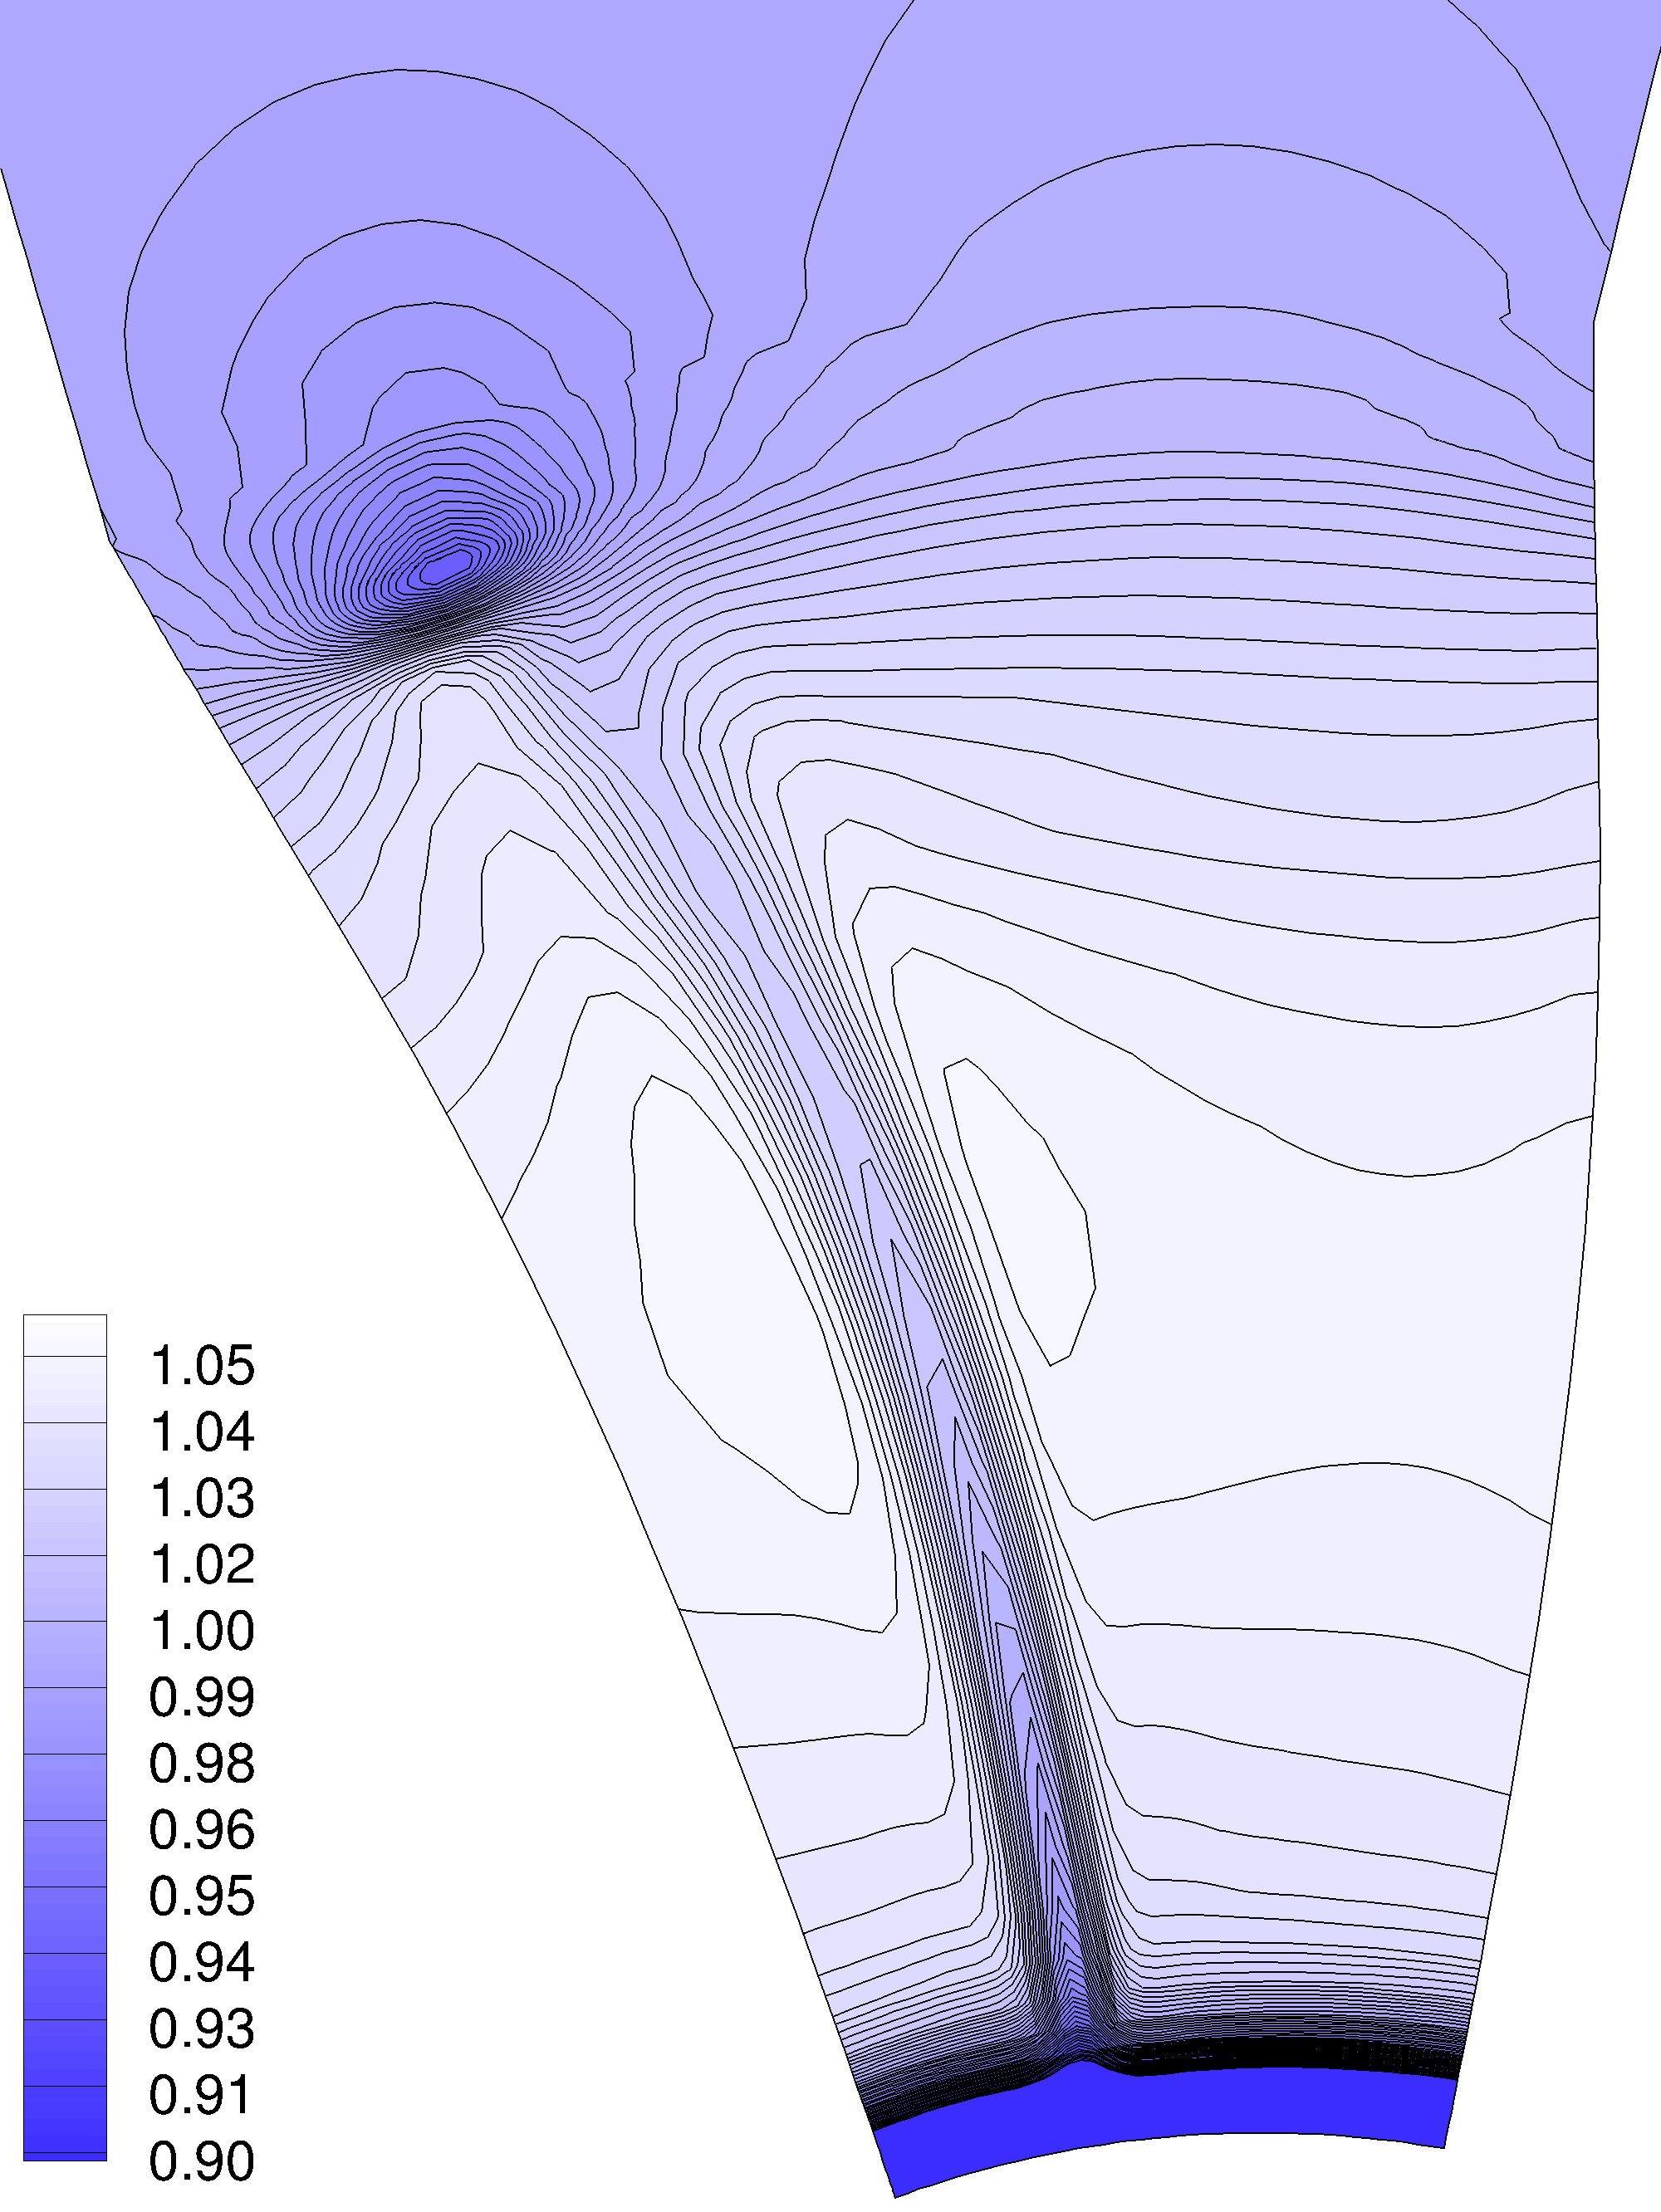
\includegraphics[width=.2\textwidth]{dream_hs_roe2.png}}
  \subfigure[\aipx-HS]{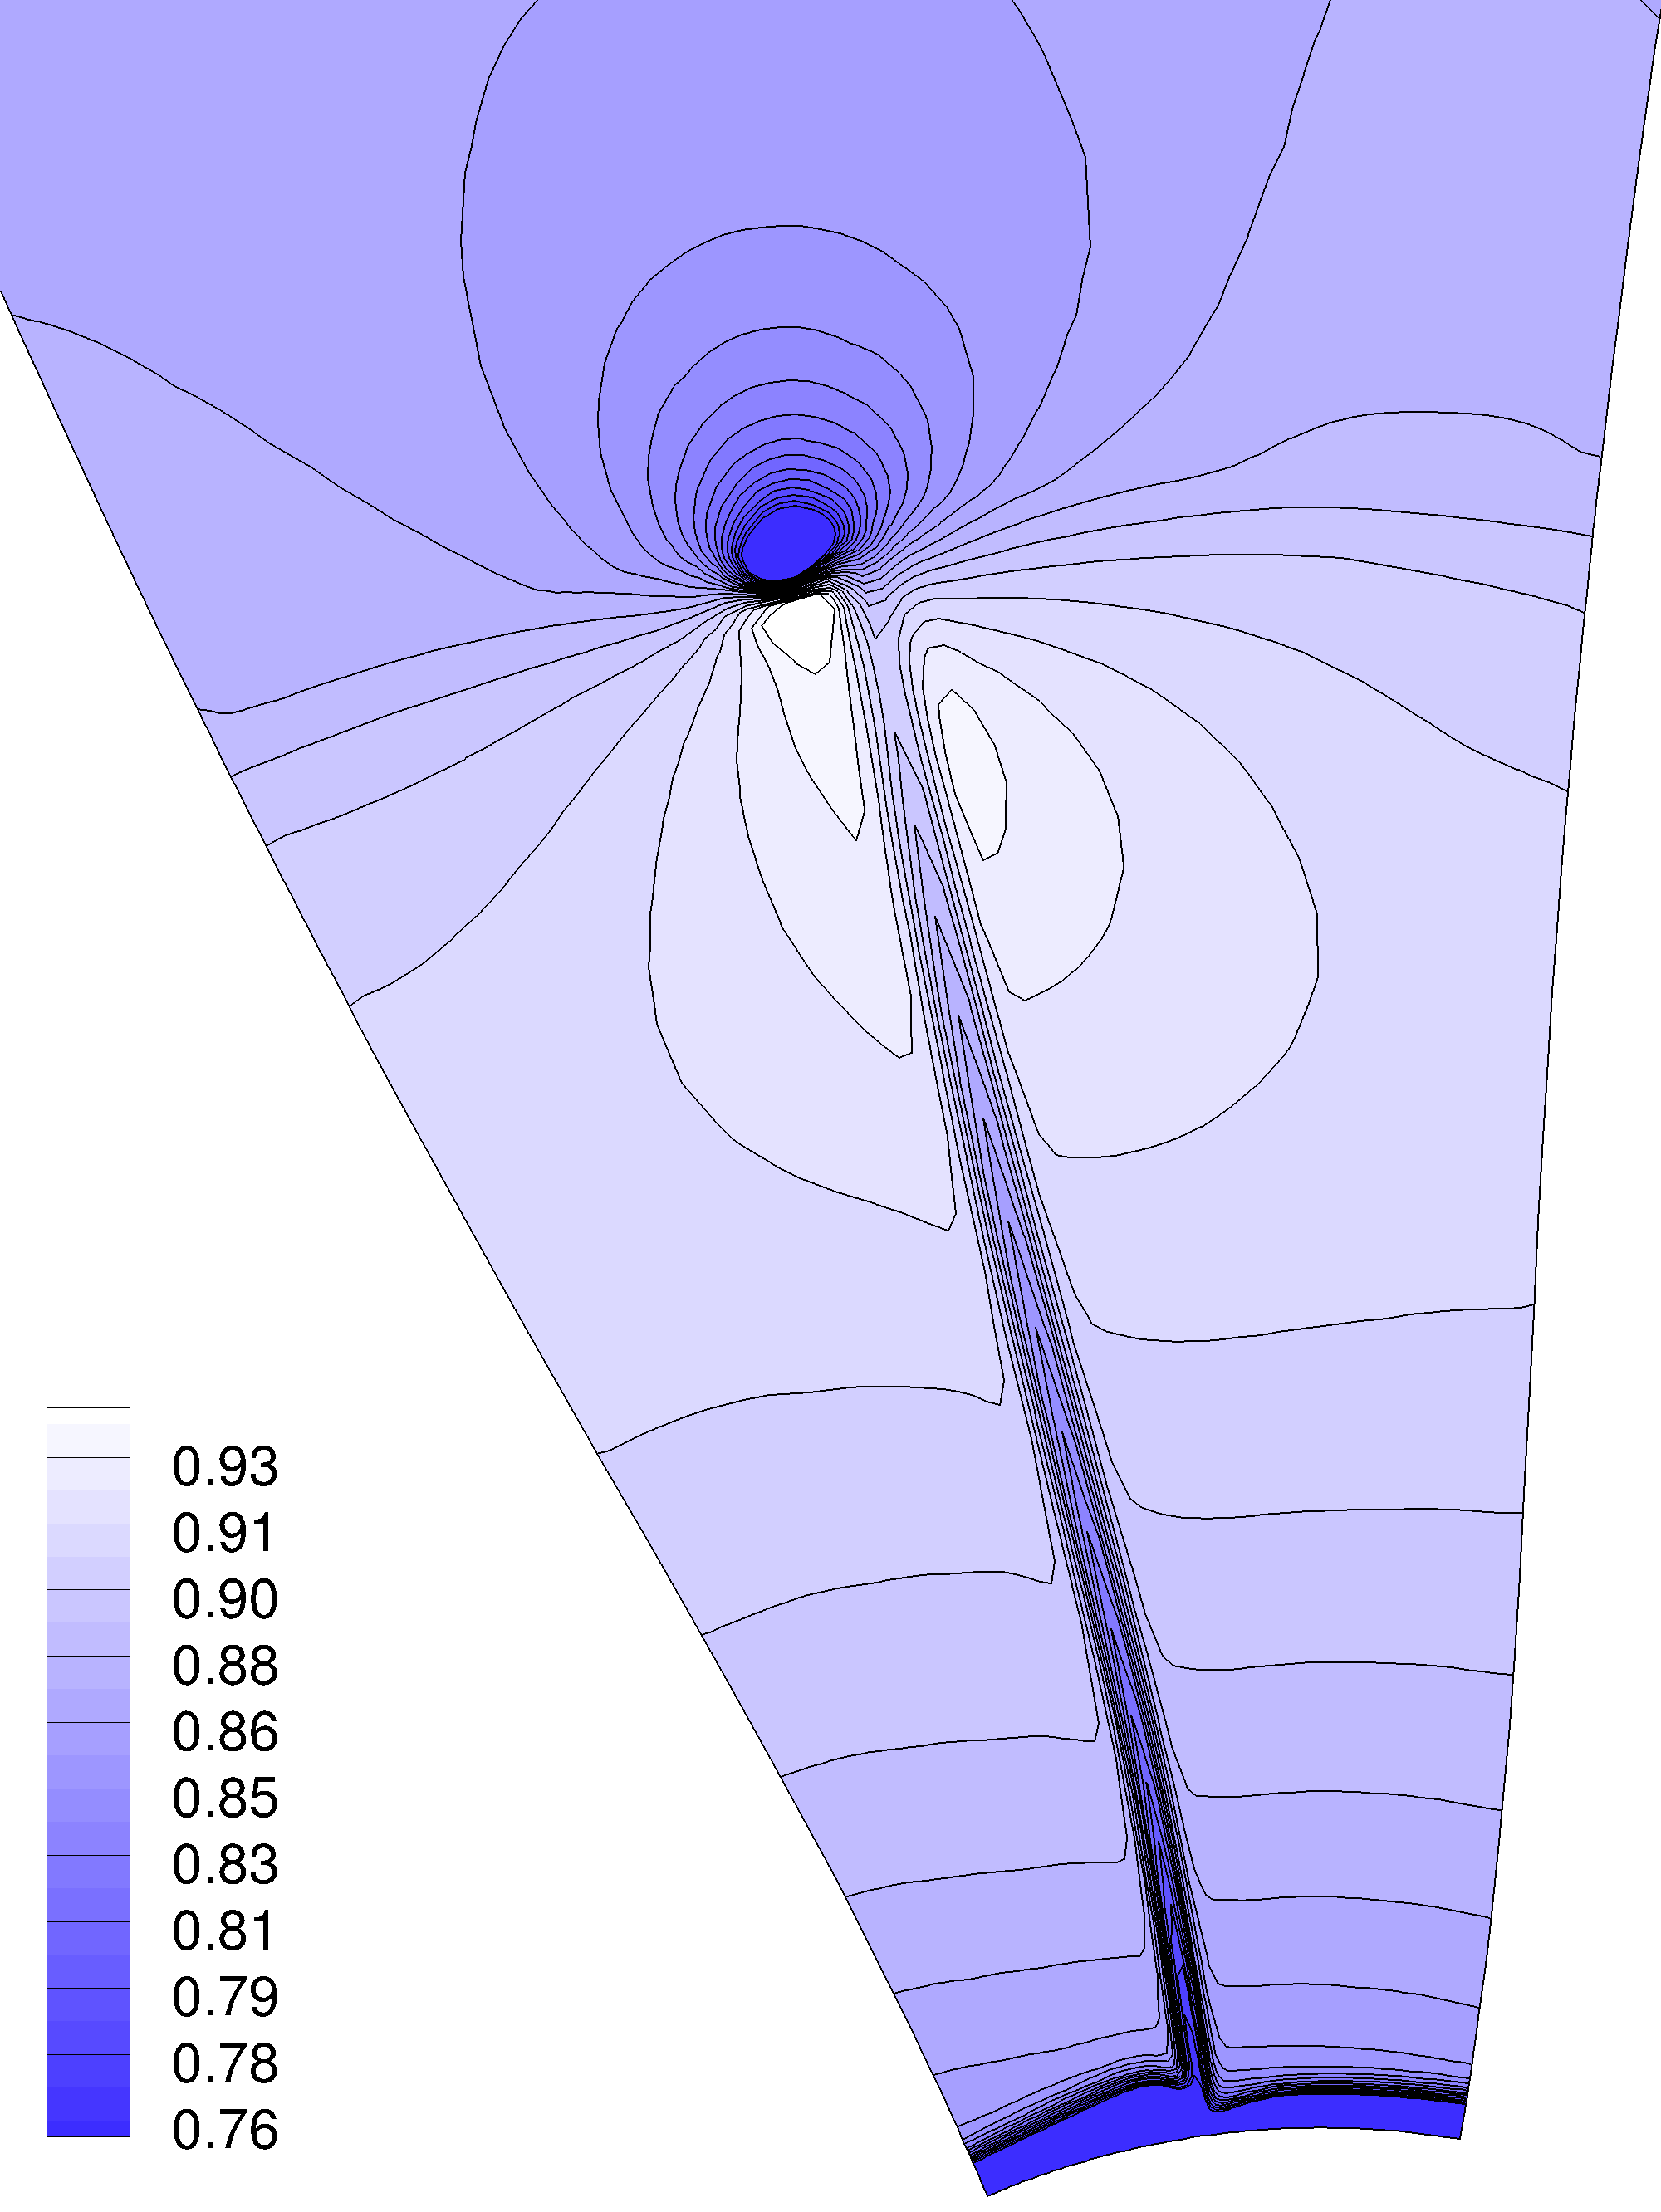
\includegraphics[width=.2\textwidth]{aipx7_hs.png}}
  \caption{Non-dimensional axial momentum $(\rho U)/(\rho U)_\infty$ 
  at the rotor/rotor interface (mixing-plane computations).}
  \label{fig:crorroxvmap}
\end{figure}